\chapter{ZCal - calibrating radio interferometric data with machine learning}
\label{c3}
ZCal, in full "Zitha calibration" is a new machine learning radio data calibration experiment through which one makes use of the telescope sensor data to determine the relationship with calibrator solutions obtained using conventional calibration techniques. In Section \ref{Exp}, we further discuss the external parameters affecting the observed radio interferometric data, followed by a brief description of the KAT-7 telescope and  Section \ref{kat7} describes how the sensor data and calibration solutions are processed for training. In Section \ref{algo1} we define and describe the regression algorithms used for our experiment, and in Section \ref{TT} we describe the training and testing procedure of the algorithms leading to the output results of our experiment in Section \ref{sec3}. 
\section{External parameters affecting the data}
\label{Exp}
%%Each antenna in an array has a primary beam which is used for perfect resolution during an observation of a source. The resolution of each antenna is defined as =1.22 / D, where  ~ 21 cm is the  wavelength, D is the diameter of your dish and is the resolution angle. In an interferometric array of N antennas with baselines b, the resolution angle is defined as  =1.22  / d, where d is the maximum baseline in an array.   The beam of all the baselines is call a synthesised beam which is a multiplication of all the primary beams.

Astronomical observations done with interferometric radio
telescopes suffer from various variable gain effects. The more the instrument, the more complex the gain effects the astronomers are likely to deal with. These can
broadly be classified as direction-independent and direction-dependent errors. The complex instrumental gains due to the electronic devices in the telescope such as the receiver elements are directionally independent \citep{bhatnagar2008correcting}; as well as the tropospheric amplitude and phase effects; relative amplitude and phase gain for each antenna; amplitude response as a function of elevation (gain curve) and phase and amplitude drifts in the electronics of each antenna\citep{bhatnagar2008correcting}.

As defined in Chapter 1, \textit{calibration} is the process of correcting for the signal corrupted by various mechanisms. Some of these mechanisms include external parameters such as fluctuations in air temperature, weather conditions on site and antenna pointing errors \citep{taylor1999synthesis}. The antenna pointing error is the difference between the actual pointing position  of the telescope and the requested (to go) position. Though an array consists of more than one antenna, each with a tracking centre, during a request ("POINT"), they must all follow the same required position. However, this is not always accurate, owing to misalignment of the elevation axis, atmospheric refraction, gravitational deformation of the structure, differential heating of the structure and wind loading \citep{taylor1999synthesis}. Wind loading is an effect that degrades the pointing accuracy, thus the design of the telescope structure plays a role in terms of wind loads \citep{smithdynamic}. Telescopes with a large dish structure are subjected to large wind loads. The wind speed and the geometric dimensions are the cause of highly turbulent flows around the antenna. There are violent shifts in airflow on the surface and around the antenna \citep{upnere2012characterization}. The following equation \ref{sens} shows the nominal expected sensitivity of the telescope without any errors:
\begin{align}
\left[\frac{2kT_{sys}}{A_{eff}\sqrt{N(N-1)\tau \Delta \nu}}\right]
\label{sens},
\end{align}
 where ($N$ is the number of antennas in the array,  $A_{eff}$ is aperture efficiency, $\tau$ is the integration time, $k=1.38\times 10^{-23}Jk^{-1}$ is the Boltzmann constant, $\Delta \nu$ is the bandwidth and $T_{sys}=\sum T_{i}$ an additive of noise contribution from different source such as atmosphere, ground, telescope surface and receivers) \citep{wilson2013tools}. 



\section{KAT-7 telescope}
\label{kat7}

\begin{figure}[H]
  \centering
    \includegraphics[width=0.6\textwidth]{images/K7.png}
    \caption{The seven-dish MeerKAT precursor array, \citep{carignan2013kat}}
  \label{images/kat7.png}
\end{figure}

The KAT-7 is a seven-dish interferometry that was built as an engineering prototype for  techniques and technologies in preparation for the 64-dish Karoo Array Telescope (MeerKAT). These instruments are located in the Northern Cape Karoo desert region and are operated remotely from CapeTown. The construction of  KAT-7 began in
2008 with the writing of the telescope requirements specification and was completed in 2010.  It was then operated in engineering (commissioning) mode until its shut-down in 2016 \citep{foley2016engineering}. As seen in Table \ref{images/kat7.png}, KAT-7 antennas are extremely close together with baseline ranging between 26 and 185 m \citep{carignan2013kat}. More parameter specifications are presented in the Tables \ref{DSpec} and \ref{DSpec}:
\begin{table}[H]\centering
\begin{tabular}{l l }
\toprule
\textbf{Parameter} & \textbf{Value}\\
\midrule
Dish diameter&12 m \\
Number of antennas& 7\\
Min baseline & 26 m\\
Max baseline & 185 m\\
Frequency range & 1200-1950 MHz\\
Max instantaneous bandwidth &256 MHz\\
Polarization   & Linear H $\&$ V\\
Systems temperature ($T_{sys}$) & $<$35 K across the entire frequency band\\
Aperture effeciency & 0.65\\
Location &  latitude 30.7148$^{\circ}$ S, longitude 21.388 $^{\circ}$ E\\
cryogenic temperature on receiver & 80 K\\
Digital back end & Roach \\
Elevation & 1054 m\\
\bottomrule
\end{tabular}
\caption{The instrument consists of 7 12-m dishes with linearly polarized feeds. The operational lower noise amplifier for each dish is $80\;K$  with system temperature $<35\;K$. The frequency range of this instrument is $1200-1950 \text{MHz}$ with bandwidth of $256\;\text{MHz}$ \citep{foley2016engineering}.}
\label{K7 spec}
\end{table}

%\begin{table}[H]\centering
%\begin{tabular}{l l l l}
%\toprule
%\textbf{Mode}& \textbf{Total BW(MHz)} & \textbf{Number of chan} & \textbf{Chan width(KHz)} \\
%\midrule
%c16n2M4k  &  1.5625	& 4096& 	0.381\\
%c16n7M4k & 6.25 & 	4096& 	1.526\\
%c16n25M4k& 	25&	4096& 	6.104\\
%c16n400M4k&  256& 	1024& 	390.625\\
%\bottomrule
%\end{tabular}
%\caption{The table is showing different correlator modes for observations. The correlator is based
%on the so-called 'FX, architecture, i.e (Fourier transform 'F' followed
%by Cross-correlation 'X'). The F  which channelise the incoming data streams
%into spectral components and the X does the multiplication and accumulation of each and every product pair \citep{foley2016engineering}.}
%\label{K7 modes}
%\end{table}
\begin{table}[H]\centering
\begin{tabular}{l l }
\toprule
\textbf{Parameter} & \textbf{Value}\\
\midrule
Pointing accuracy & 25 $^{\prime \prime}$ \\
Wind (Operational) & 36 km/h\\
Wind (Marginal Operation) km/h & 45 km/h\\
Wind (Drive to Stow) & 55 km/h\\
Wind (Survival) & 160 km/h\\
Azimuth Rotation slew speed &  2$^\circ$/s\\
Azimuth limits & -175$^{\circ}$, +285 $^{\circ}$\\
Elevation slew speed & 1$^{\circ}$/s\\
Elevation limits & 0$^{\circ}$, 90 $^{\circ}$\\
Feed/Cryo & Mass 75 kg\\
\bottomrule
\end{tabular}
\caption{The table shows the KAT-7 dish specification \citep{foley2016engineering}.}
\label{DSpec}
\end{table}

\subsection{Sensor data}

During scientific observations, data indexed by time are continuously collected from instruments and  environment (atmospheric pressure, air temperature,  wind conditions, and relative humidity, wind direction, etc). Samples as a function of time are recorded from software and sensors attached to the telescopes with their adjoining instrumentation \citep{slabberICALEPCS2017}. Sampling strategies are set on sensors processed by the control and monitoring (CAM) system, ranging from several updates per second to infrequent updates. The typical sample in KAT-7 CAM contains the following attributes: a sensor name, sample timestamp, value timestamp, status and a value as shown in the following example, where red represents the sensor sample and green is the sensor sample description  \citep{slabber2015overview, slabber2015illustrate}. 

\definecolor{keywords}{RGB}{255,0,90}
\definecolor{comments}{RGB}{0,0,113}
\definecolor{red}{RGB}{160,0,0}
\definecolor{green}{RGB}{0,150,0}
 
\lstset{language=Python, 
        basicstyle=\ttfamily\small, 
        keywordstyle=\color{keywords},
        commentstyle=\color{comments},
        stringstyle=\color{red},
        showstringspaces=false,
        identifierstyle=\color{green}}

\begin{tcolorbox} 
\begin{lstlisting}

   {"name": wx_station_wind_speed,
   "time": 1506430493.4778199196,
   "status": nominal,
   "value_ts": 1506430493.4774999619,
   "value": 10.3}

   #SENSOR_NAME A normalised form of a sensor name.

   #SAMPLE_TS The UNIX timestamp of when the sample was
   #first processed by the CAM system.

   #VALUE_TS A UNIX timestamp when the acquisition
   #was performed. 

   #STATUS indicate the state of the sensor when
   #the sample was taken. Can have a value of UNKNOWN,
   #WARN, NOMINAL, FAILURE, INACTIVE, ERROR, UNREACHABLE. 
\end{lstlisting}
\end{tcolorbox}

All the telescope components are interfaced to the CAM system via the Karoo Array Telescope Communication Protocol (KATCP), i.e KATCP is responsible for internal communication between CAM components and other subsystems (science data processing, correlator beamformer, etc) \citep{slabber2015overview}. A KATCP interface exposes requests and sensors. To access the sensor information for analysis, users from different subsystems  would  connect to the CAM webserver using Python client and subscribe to sensor data of interest. 

\subsection{Preparation of training data}\label{prep}

The objective of this study is to find correlations between
calibration solutions and sensor information on the telescope.
Therefore the main dataset for the study is the time-based
sensor information of each antenna.
The process of data collection encompasses all of the steps required to obtain the desired data in digital format. Methods of data collection include acquiring and archiving new observations, querying existing databases according to the science
problem at hand, and performing as necessary any cross-matching or data combining  \citep{ball2010data}.

%In this chapter we will look at modelling the behaviour patterns of individual antennas and calibration steps based on Karoo Array Telescope (KAT-7) \ref{images/kat7.png}.

In every observation, the collected data are stored by the data capturing system in the Hierarchical Data Format (HDF5), which is a set of file formats designed to store and organize large amounts of data. The HDF5 file consists of two parts meta-data and observed visibilities. In meta-data one finds static information of the data set, including observer, dump rate and all the available subarrays and spectral windows in the data set selection criteria (antennas, channel frequencies, targets, scan information) and sensor data of interest as a function of time. The data observed by the radio telescope are in the  form of complex numbers referred to as visibilities, as described in Chapter 1. Each source observed contains its own visibilities as a function of time along with sensor data,  which keep a record of the telescope's activity and behaviour as these are observed.

In preparation for the training and testing dataset, we look at environmental sensors and instrumental sensors
recorded during observations with a flux calibrator and a phase calibrator source
PKS1613-586 in Figure \ref{pks1613}. This was the most frequently used phase calibrator during the KAT-7 commissioning phase. A series of observations for different tests with this calibrator \ref{pks1613} were taken in the period from December 2011 to November 2014. These tests includes Circinus X-1 monitoring at frequency $2022 - 1622.391 \;\text{MHz}$; OH maser monitoring at frequency $1666.481 - 1664.919 \;\text{MHz}$, $1666.381-1666.819\;\text{MHz}$,  $1666.281- 1664.719\;\text{MHz}$; spectral dynamic range test at frequency $1669.125 - 1662.877 \;\text{MHz}$, $1678.500 - 1653.506 \;\text{MHz}$; Circinus X-1 H absorption at frequency $1425.125 - 1418.827\; \text{MHz}$, $1424.125 - 1417.877 \;\text{MHz}$ and imaging new calibrators at frequency $2022 - 1622.391 \;\text{MHz}$. The chosen sensors of interest from each observation are: 
\begin{enumerate}

\item Air temperature
\item Wind speed
\item Wind direction 
\item Air pressure 
\item Relative humidity 
\item Actual refraction elevation
\item Actual refraction azimuth
\item Actual scan elevation
\item Actual scan azimuth 
\item Actual pointing elevation
\item Actual pointing azimuth. 
\end{enumerate}
The environmental sensors measure the environmental conditions on site via the weather station installed around the telescope and the instrumental sensors (pointing) record the pointing azimuth and elevation activities of a telescope. These are examples of how each environmental and instrumental sensor are represented per antenna X.

\definecolor{keywords}{RGB}{255,0,90}
\definecolor{comments}{RGB}{0,0,113}
\definecolor{red}{RGB}{160,0,0}
\definecolor{green}{RGB}{0,150,0}
 
\lstset{language=Python, 
        basicstyle=\ttfamily\small, 
        keywordstyle=\color{keywords},
        commentstyle=\color{comments},
        stringstyle=\color{red},
        showstringspaces=false,
        identifierstyle=\color{green}}
        
        
\begin{tcolorbox}
\begin{lstlisting}
   {"name": anc_air_pressure,
   "time": 1506430493.4778199196,
   "status": nominal,
   "value_ts": 1506430493.4774999619,
   "value": 981.65}
   
   {"name": anc_gust_wind_speed,
   "time": 1506430493.4778199196,
   "status": nominal,
   "value_ts": 1506430493.4774999619,
   "value": 3.96}

   {"name": "anc_air_temperature",
   "time": 1506430493.4778199196,
   "status": "nominal",
   "value_ts": 1506430493.4774999619,
   "value": 23.96}

   {"name": anc_air_relative_humidity,
   "time": 1506430493.4778199196,
   "status": nominal,
   "value_ts": 1506430493.4774999619,
   "value": 25.87}

   {"name": anc_wind-direction,
   "time": 1506430493.4778199196,
   "status": nominal,
   "value_ts": 1506430493.4774999619,
   "value": 46.61}
\end{lstlisting}
\end{tcolorbox}

\begin{tcolorbox}
\begin{lstlisting}
   {"name": antX_pos.actual-pointm-elev,
   "time": 1506430493.4778199196,
   "status": nominal,
   "value_ts": 1506430493.4774999619,
   "value": 89.97}
   
   {"name": antX_pos.actual-pointm-azim,
   "time": 1506430493.4778199196,
   "status": nominal,
   "value_ts": 1506430493.4774999619,
   "value": -78.81}
   
   {"name": antX_pos.actual-refrac-elev,
   "time": 1506430493.4778199196,
   "status": nominal,
   "value_ts": 1506430493.4774999619,
   "value": 89.80}
   
   {"name": antX_pos.actual-refrac-azim,
   "time": 1506430493.4778199196,
   "status": nominal,
   "value_ts": 1506430493.4774999619,
   "value": -70.15}
   
   {"name": antX_pos.actual-scan-elev,
   "time": 1506430493.4778199196,
   "status": nominal,
   "value_ts": 1506430493.4774999619,
   "value": 89.82}
   
   {"name": antX_pos.actual-scan-azim,
   "time": 1506430493.4778199196,
   "status": nominal,
   "value_ts": 1506430493.4774999619,
   "value": 78.94}
   
\end{lstlisting}
\end{tcolorbox}

We access this data from the HDF5 file using the KAT-7 data access library called katdal \citep{skatelescope}. We select the sensor data of interest with time index during the telescope tracking of the flux calibrator and phase calibrator PKS1613-586. The following is a Python code example showing how the sensor time index is selected from the observations for a specific calibrator.

\begin{tcolorbox}
\begin{lstlisting}
#importing data access library
import katdal
import numpy
import time

#Opening the observation file 
hdf5=katdal.open('1329697773.h5')
#Selecting data of interest from the the observation file
hdf5.select(scans='track',
            targets=['PKS1934-63','PKS1613-586'],
            channels=slice(199,800)
            )   
#Obtaining sensor timestamps            
h5df5_timestamps=[]
temp_time = np.empty((len(h5.timestamps)))
for i in range(0,len(h5.timestamps)):
    temp_time[i]=(h5.timestamps[i])
    timeh5.append(T.ctime(temp_time[i]))      
       
#Selecting time during the scan of the calibrators
Time_Scan=[]
for scan in hdf5.scans() :
    #Taking average of start and endtime scan of calibrator source
    Average=((hdf5.timestamps[0]+
              hdf5.timestamps[len(hdf5.timestamps)-1])/2
             ) 
    Time_Scan.append(time.ctime(Average))
    
#obtaining time index of telescope sensors and scan time.
Time_index=numpy.where(np.in1d(numpy.unique(h5df5_timestamps),
                       Time_Scan))[0]
                       
                                           
\end{lstlisting}
\end{tcolorbox}

 The katdal library can manipulate the HDF5 observation file in many ways, including file format conversion from HDF5 to measurement sets (MS). This option is useful for astronomers using CASA for data calibration and visualization \citep{foley2016engineering}. This conversion also provides an option whereby one flags all channels affected with known radio frequency interference (RFI). Once the observation file has been converted to ms format, hand flagging for unknown RFI is performed inside CASA using the task $\textit{flagdata}$ for H and V cross correlation products. After satisfactory flagging of the data, one then proceeds to the calibration step. 
 
The systematic time-dependent complex gain errors denoted by $J_{ij}$ (where $i,j$ represent the baseline of two or more antennas) are the most dominant calibration effect in the visibility data, and a solution for them is necessary before proceeding with any other calibration \citep{ott2013casa}. In this dissertation we only focus on the 1GC calibration with an interest in obtaining complex gain calibration solutions for the phase calibrator PKS1613-586. In the process of 1GC, as explained in chapter 1, the complex gain calibration ($\textit{gaincal}$)  CASA task determines the time-based complex antenna gains solutions $G$ (amplitude and phase) for each polarization H \& V and each spectral window, from the visibility data of the specified phase calibration source PKS1613-586 and stores these in calibration tables.
 
These solutions are calculated based on reference antenna 5 in our case, since it is an antenna that is reasonably close to the center of the array and it was known to be particularly stable with no drop-outs during KAT-7 commissioning \citep{ott2013casa}. The task $\textit{gaincal}$ in CASA factors $J_{i,j}$ into antenna-based components, so one does not see a set of values for each baseline, but rather only one for each antenna ($J_i$) \citep{editioncasa}. 

Since our phase calibrator PKS1613-586 has an unknown flux density, the obtained values of the antenna based amplitude solutions differ from the correct ones by a factor depending only on the true source flux density by 

\begin{equation}
\frac{1\;\mathrm{Jy}}{(\text{true source flux density})^{0.5}},\;  \text{where 1 $\mathrm{Jy}$ is the assumed flux density for \text{PKS1613-586}}.
\end{equation} 

We then used one of the following flux-density calibrators with known flux models: PKS1934-63, 3C147, 3C286 tied to the Perley-Taylor 99 to scale the correct gain amplitude of the phase calibrator in Figure \ref{pks1613} so that it match the scale amplitude solutions for the flux-density calibrators as well as possible by running the CASA task $\textit{fluxscale}$ \citep{editioncasa}. This process is called $\textit{bootstrapping}$. After obtaining the final table with correct amplitude and phase complex gain solutions for the phase calibrator in Figure \ref{pks1613}, we then used the complex solutions matrix written to the "CPARAM" column to generate the training and testing calibration solution data per antenna $i$. An example of the complex gain amplitude and phase solutions is shown in Figures \ref{amp} and \ref{phase}. These solutions were obtained using the CASA task $gaincal$ described in Chapter 1. 

The following code shows how the parameters were set in standard practice of 1GC as described in chapter 1 section \ref{caltech}.

\begin{tcolorbox}
\begin{lstlisting}
#Set flux for flux calibrator
default(setjy)
vis = msfile
field = flux_calibrator
fluxdensity  = -1
standard = 'Perley-Taylor 99'
setjy()

#Bandpass calibration
default(bandpass)
vis = msfile
caltable = bandpasstable
field = flux_calibrator
refant = reference_antenna
solnorm = True
combine = 'scan'
solint = 'inf'
bandtype = 'B'
minsnr = 5
interp = ['nearest']
bandpass()
\end{lstlisting}
\end{tcolorbox}
\begin{tcolorbox}
\begin{lstlisting}
#Calculating G solution for flux calibrator 
default(gaincal)
vis = msfile
caltable = gaintable
field = flux_calibrator
solint = 'inf'
refant = reference_antenna
gaintype = 'G'
calmode = 'ap'
solnorm = False
minsnr = 5
gaintable = [bandpasstable]
interp = ['nearest']
gaincal()
  
#G solution for gain calibrator
default(gaincal)
vis = msfile
caltable = gaintable
field = gain_calibrator
solint = 'inf'
refant = reference_antenna
gaintype = 'G'
calmode = 'ap'
append=True
solnorm = False
minsnr = 5
gaintable = [bandpasstable]
interp = ['nearest']
gaincal()   

#Scaling flux density for phase calibrator
default(fluxscale)
vis = msfile
caltable = gaintable
fluxtable = fluxtable
reference = flux_calibrator
transfer = gain_calibrator
fluxscale()
\end{lstlisting}
\citep{editioncasa}
\end{tcolorbox}

A multi-frequency synthesis image deconvolution was carried out using the $\textit{CLEAN}$ CASA task with an image size of  $256 \times 256$ and cell size of $30$ arc seconds. The image rms noise in Figure \ref{pks1613} was measured using the rms noise of the 0 iteration residual image.
\begin{tcolorbox}
\begin{lstlisting}
     clean(vis='CircinusX-1.split.ms',
     imagename='PKS1613586.im',
     niter=10000,threshold='3.0mJy',
     psfmode='hogbom',
     interactive=False,
     imsize=512,
     cell='30arcsec',
     stokes='I',
     weighting='briggs',
     mode='mfs',
     usescratch=True)
\end{lstlisting}
\citep{editioncasa}
\end{tcolorbox}
 \begin{figure}[H]
 \centering
    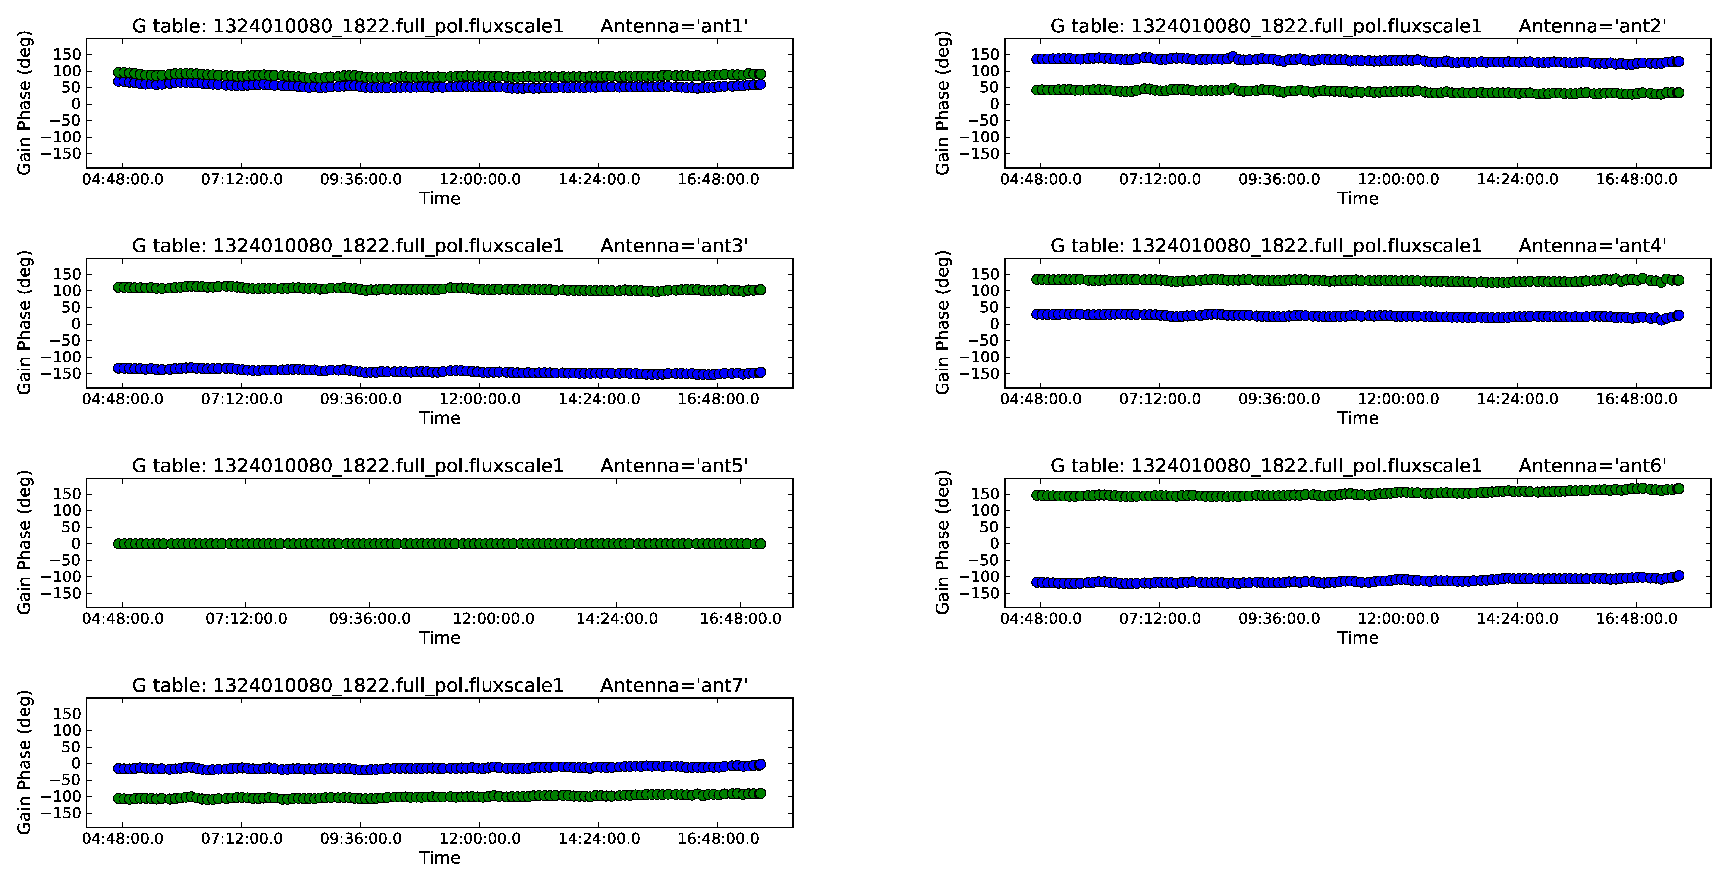
\includegraphics[ height=13cm, width=15.5cm]{images/phaseCasa.eps}
    \caption{Complex gain phase solutions for phase calibrator PKS1613-586 obtained from CASA per antenna $i$. Blue is H-polarization and green is V-polarization. Antenna 5 shows zero phase since it is used as a reference antenna.}
  \label{phase}
\end{figure}

 \begin{figure}[H]
 \centering
    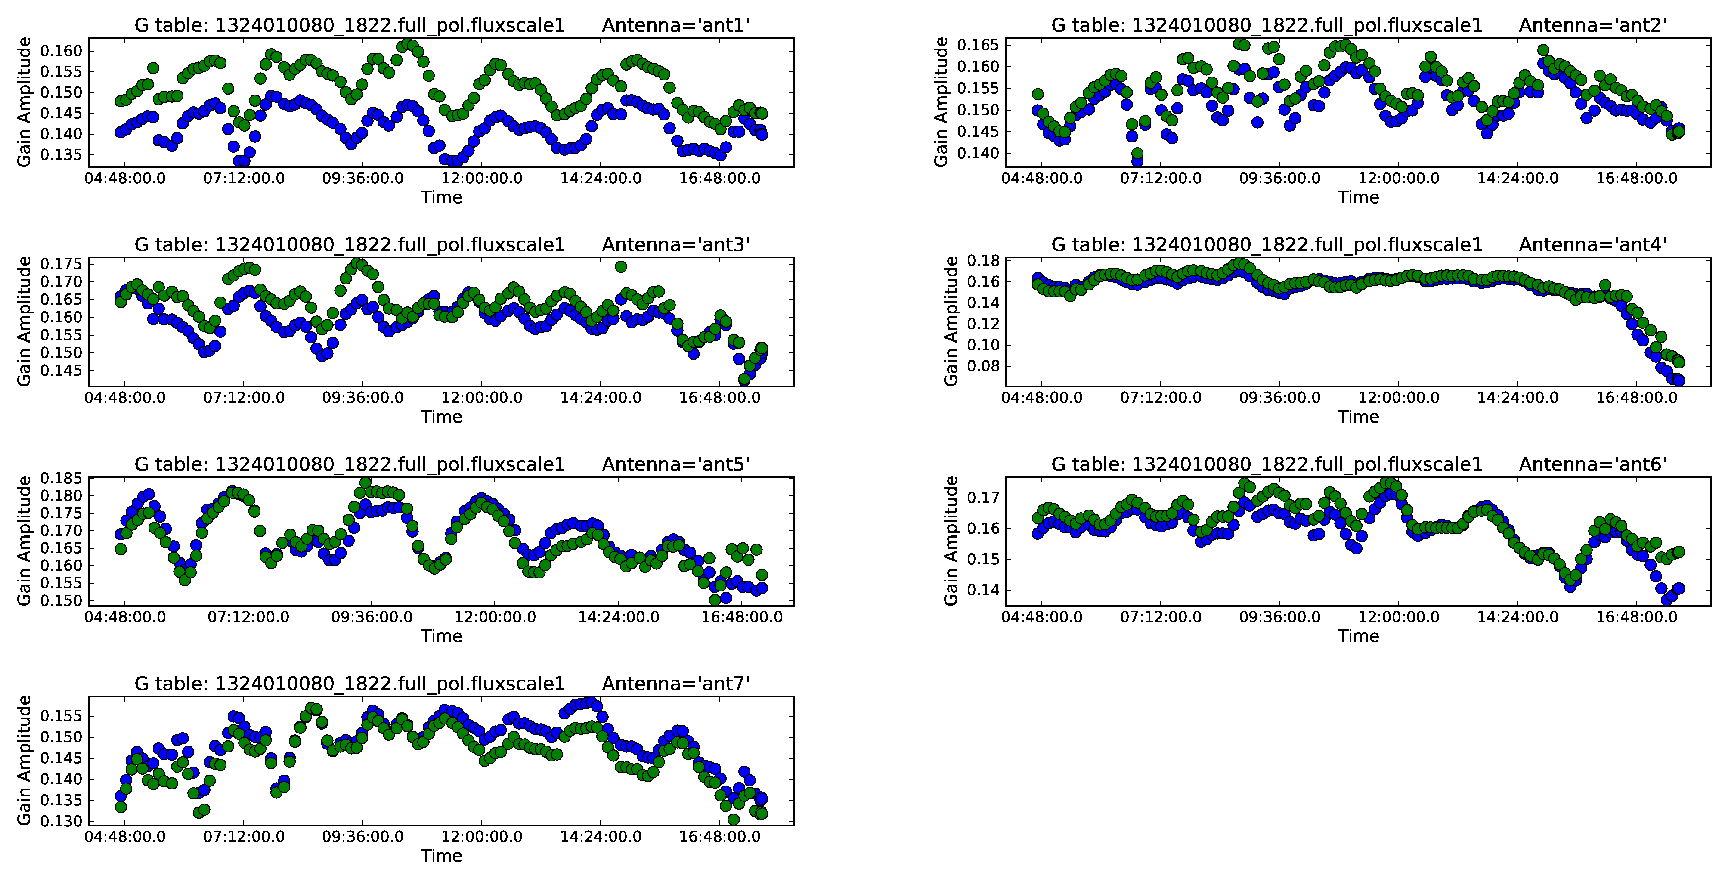
\includegraphics[ height=13cm, width=15.5cm]{images/CasaAmp.eps}
    \caption{Complex gain amplitude solutions for phase calibrator PKS1613-586 obtained from CASA per antenna $i$. Blue is H-polarization and green is V-polarization. }
  \label{amp}
\end{figure}
 
 \begin{figure}[H]
 \centering
    \includegraphics[ height=8cm, width=10cm]{images/162.png}
    \caption{An image of the phase calibrator PKS1613-586 located at RA, Dec (J2000): 16:17:17, -58:48:07. Its flux density in $\mathrm{Jy}$ at $\text{frequency}=1.83 \mathrm{GHz}$ is $4.6 \pm 0.015$. This flux scaling was carried out in CASA using a strong flux calibrator. The expected rms noise of this image was calculated to be 0.08$\mathrm{Jy}$ using $\textit{CLEAN}$ task in CASA.}
  \label{pks1613}
\end{figure}

\section{Training and testing}
\label{TT}
The process of training and testing involves feeding a learning algorithm with training data (seen data) to learn from by finding suitable parameters and evaluate its performance using testing data (unseen), as illustrated in Figure \ref{overview}. A fundamental assumption of machine learning is that the distribution of the training data are the representative from which future data will be chosen \citep{witten2016data}. Each instance in the training set contains "target value" and several "attributes" (namely features). 

\begin{figure}[H]
  \centering
    \includegraphics[width=0.7\textwidth]{images/MLSampler.png}
    \caption{An overview of machine learning model training \citep{flach2012machine}.}
  \label{overview}
\end{figure}

Referring to Section \ref{prep}, some challenges and difficulties of gathering  a larger data set were encountered  due to faulty radio telescopes leading to observations being conducted with fewer elements in an array, observations with target of interest PKS1613-586 conducted using only the baselines of interest (short or long), KAT-7's lifespan lasting for a short period, and radio frequency interference affecting calibration solutions. The advantage of having a large testing dataset is a more reliable estimate of accuracy, whereas a large training set is more representative of how much data are available for the learning process. 

Despite the challenges mentioned above, we managed to construct a data matrix $\textbf{M}$ of dimension  $1760\times 75$ containing sensor data $\textbf{X}_t\in \mathbb{R}^{1760 \times 47}$ and 1GC calibration solutions $\textbf{Y}_t$ $\in \mathbb{C}^{1760 \times 14}$ from 28 different observations at integration time $\Delta t$ ranging from $1-12$ hours dependending on each observation requirement. Take note that the 14 columns in plane $\mathbb{C}$ represent the amplitude and phase solutions for H,V polarization, i.e. $7 \times 2$; and the 47 columns in plane $\mathbb{R}$ are the number of selected sensors for all the antennas. Since each calibration solution in $\textbf{Y}_t$ is represented as a complex variable \begin{align}
Ae^{i\phi}= A(\cos\phi + i\sin\phi), \label{cx}
\end{align} for each polarization H $\&$ V. Due to different physical causes on the received signal, we therefore choose to treat the antenna phases and amplitudes separately by splitting equation \ref{cx}, into gain amplitude solutions  $\left|Ae^{i\phi}\right|$ and gain phase solutions $\phi$ in radians for both H $\&$ V. In every supervised machine learning problem, it is crucial to label the input and output of the dataset before starting the learning process. In our case, since this is a regression problem aiming to predict calibration solutions from sensor data, we therefore label the sensor data as input features and the calibration solutions as output targets.
    
\begin{figure}[H]
  \centering
    \includegraphics[width=0.7\textwidth]{images/cal4.png}
    \caption{Observation procedure and calibration using CASA}
  \label{Cal2}
\end{figure}

\begin{figure}[H]
  \centering
    \includegraphics[width=0.7\textwidth]{images/Cal3.png}
    \caption{Observation procedure goal using machine learning}
  \label{Cal3}
\end{figure}

Figure \ref{Cal2} shows the observation procedure of KAT-7 where the calibrator is close to the target source (preferably within the range of $10^{\circ}$ to $15^{\circ}$), with the scan switching  between  the target and the calibrator \citep{taylor1999synthesis}. This is to minimize the phase perturbation caused by atmosphere. The calibration solutions are obtained from the phase calibrator ("green") in Figure \ref{Cal2} at different time intervals $\Delta t$ of tracking called duty cycles. This is done assuming that the calibrator PKS1613-586 has invariant characteristics (i.e. known positions in the sky or known properties from previous observations). One of the standard properties for an ideal instrument would be the $0^{\circ}$ antenna-based gain phase response and constant amplitude for all baselines. In reality this is not always the case because of instrumental defects such as phase and amplitude drifts in the electronics of each antenna; amplitude response as a function of elevation (gain curve), and tropospheric amplitude and phase effects and other external effects. Hence, to calculate the calibration solutions, CASA considers each antenna-based gain $J_i$ and the prior information about the calibrator to perform some adjustments or estimations $G$ over the calibrator's duty cycle $\Delta t$ for all the instruments $i,j$. These solutions at each duty cycle are then temporarily interpolated using the $\textit{interp}$ parameter inside the $\textit{gaincal}$ CASA task. 

%Interpolation is a model based recovery of continuous data from discrete data with known range \citep{thevenaz2000image}. There are different methods of interpolation used, and in this Section, we only look at linear and nearest interpolation which are popular in radio calibration. Example: Assume that we have two known data points $(x_1,y_1,t_1)$ and  $(x_2,y_2,t_2)$ at time $t_1$ and $t_2$, we would like to estimate what $y$ value we would obtain at time $t$ for some point $x$ that is between $x_1$ and $x_2$. For nearest interpolation method, $y$ would be assigned to the value of the nearest point of $x$. For linear interpolation method, a line is fitted between the points $(x_1,y_1,t_1)$ and $(x_2,y_2,t_2)$  and we look to see the value of $y$ in a line for our chosen $x$ at time $t$. The points $x_1,\dots, x_n$ are called the interpolation points. The property of passing
%through these points is referred to as interpolating the data and the function that interpolates the data is an interpolant \citep{levy2010introduction}. An example of interpolation is further illustrated in the following Figure \ref{int}. 
%
%  \begin{figure}[H]
%  \centering
%    \includegraphics[width=0.5\textwidth]{images/Int.png}
%    \caption{Given a function $f(x)$ with distinct points $x_0<x_1,<x_2,\dots <x_n$ at $n+1$. The interpolation problem is to construct a function $Q(x)$ that passes through these points, i.e, to find a function $Q(x)$ such that the requirements $Q(x_i)=f(x_i)$, $0\leq i\leq n$ are satisfied \citep{levy2010introduction}.}
%  \label{int}
%\end{figure}
 
After obtaining solutions $G$, they are written into calibration tables and later applied to the target source of interest, $T$. The CASA task for this process is called $\textit{applycal}$, which reads the specified calibration tables, applies them to the observed data column through an interpolation process at each single time unit for different target duty cycles $\Delta t, \Delta t_{n+1},\dots$, following the order shown in Figure \ref{Cal2}. The calibrated results are then written into the corrected column for imaging or other scientific processing \citep{ott2013casa}. Since CASA "calculates" the solutions using interpolation and estimation methods given some prior information about the calibrators, the goal of the experiment is to produce a model (based on the training data) that learns the behaviour and changes of the calibrator owing to various external effects and able to predict the calibration solutions of the test data with high accuracy, given only the test sensors at different duty cycles. This will help in speeding up the calibration processes and decreasing the time duration for tracking the phase calibrator PKS1613-586 and therefore increasing the time duration for tracking the target observed as shown in Figure \ref{Cal3}. 

Since the sensor data obtained from the radio telescope are of different scales, i.e., unstructured. a pre-processing stage before proceeding with the training of the learning algorithms is necessarily. We propose to use a scaling statistical technique called Z-score normalization or standardization. This technique gives the normalized values or range of data from the original unstructured data using the concept of mean and standard deviation \citep{patro2015normalization}. The features are rescaled such that they have properties of a standard normal distribution with mean $\mu=0$ and standard deviation $\sigma=1$. 
\begin{align}
Z=\frac{\textbf{x}- \mu}{\sigma}
\end{align}
with mean:
\begin{align*}
\mu= \frac{1}{N} \sum_{j\in N} (\textbf{x}_j),
\end{align*}

and standard deviation:
\begin{align*}
\sigma=\sqrt{ \frac{1}{N} \sum_{j\in N} (\textbf{x}_j-\mu )^2}
\end{align*}
Normalizing the features so that they are centered around 0 with a standard deviation of 1 is not only important if one is comparing measurements that have different units, but is also a general requirement for many machine learning algorithms as this will be helpful for prediction \citep{bott2014feature}.

When training a learning algorithm  in machine learning, two main things might happen as described in Section \ref{comp}, namely overfitting and underfitting. To avoid these, we split the data into two subsets, i.e., training and testing data sets using the $\textit{scikit-learn}$ train-test split strategy \citep{buitinck2013api}. 

  \begin{figure}[H]
  \centering
    \includegraphics[width=0.7\textwidth]{images/t_s.png}
    \caption{This is a train-test split strategy where a data matrix is randomly split into training and testing  subsets.}
  \label{ts}
\end{figure}

From Figure \ref{ts}, once the data have been normalized, we perform a 80$ \%$ training and 20$\%$ testing split. The training set contains a known output and the model will learn using these data in order to be generalized to other data later on. The test dataset is used to test the model's prediction on this subset.
 
Model training in machine learning requires tuning of the  hyper-parameters that determine the behaviour of the learning algorithm and hence the performance
of the resulting model on unseen data. This involves finding the best combination of hyper-parameters with respect to the user-specified criterion \citep{buitinck2013api}. For this task, we make use of a randomized search cross-validation (RandomizedSearchCV) function by $\textit{scikit-learn}$ library. This library provides efficient and well-established machine learning tools in a programming environment that is user friendly and accessible to non-machine learning experts, and reusable in various scientific areas \citep{buitinck2013api}. In a randomized search cross-validation algorithm, not all hyper- parameters are tried out; instead it samples a fixed number of hyper-parameters from a specified probability distribution. i.e., given a set of parameters, $p_i$, each with $N_i$ different values, search all combinations $\prod_i N_i$ with random sampling.
%
%
   \begin{figure}[H]
  \centering
    \includegraphics[width=0.7\textwidth]{images/RegressionEST.png}
    \caption{Regression learning diagram showing how we built a regression model estimator by taking in an observation file as input and extracting the sensor data per calibrator scan to obtain an accurate model that predict calibration solutions.}
  \label{DD}
  \end{figure} 


  \begin{table}[H]
\begin{center}
\begin{tabular}{| c | c | c | c | c | c |  }
\hline
 \multicolumn{6}{ |c|}{\textbf{Decision tree estimator $p_i$}} \\ \hline
splitter & max features & min sample split & min sample leaf & max depth & cv\\ \hline
[best,random]&[log2& $\{p_i: 30 \leq p_i \leq 60 \}$& $\{p_i: 7 \leq p_i \leq 14 \}$  & $\{p_i: 700 \leq p_i \leq 1389 \}$ & 10\\ 
&sqrt& & &  &\\
&auto]& & &  &\\ \hline

\end{tabular}
\end{center}
\caption{Decision hyper-parameters} \label{DC_table}
\end{table}


  \begin{table}[H]
\begin{center}
\begin{tabular}{| c | c | c | c | c |  }
\hline
 \multicolumn{5}{ |c|}{\textbf{Random forest estimator $p_i$}} \\ \hline
 n-estimators &max features & max depth & min sample leaf& cv\\ \hline
$\{p_i: 100 \leq p_i \leq 1200 \}$&[log2& $\{p_i: 20 \leq p_i \leq 200 \}$  & $\{p_i: 3 \leq p_i \leq 50 \}$ & 10\\ 
&sqrt& & &  \\
&auto]& & &\\ \hline

\end{tabular}
\end{center}
\caption{Random forest hyper-parameters} \label{RF_table}
\end{table}


 \begin{table}[H]
\begin{center}
\begin{tabular}{| c | c | c | c | c |  }
\hline
 \multicolumn{5}{ |c|}{\textbf{Extremely randomized estimator $p_i$}} \\ \hline
 n-estimators &max features & max depth & min sample leaf& cv\\ \hline
$\{p_i: 100 \leq p_i \leq 1200 \}$&[log2 & $\{p_i: 20 \leq p_i \leq 200 \}$  & $\{p_i: 3 \leq p_i \leq 50 \}$ & 10\\ 
&sqrt& & &  \\
&auto]& & &  \\ \hline

\end{tabular}
\end{center}
\caption{Extremely randomized tree hyper-paramaters}\label{EX_table}
\end{table}

Note that since the random forest estimator \ref{RF_table} and extremely randomized estimator 
\ref{EX_table} are tree-based algorithms, they share the same hyper-parameters as the decision tree estimator \ref{DC_table}, where 
\begin{enumerate}
\item \textit{splitter}: is the strategy used to choose the split at decision node, with $p_i$ best representing the best split and random representing the random split.

\item \textit{max features}: defines the maximum number of features to be considered in the tree when making the best split. The best parameters $p_i$ to choose from are : 
\begin{itemize}
\item if $p_i$ is $\log_2$ then the maximum features is  $\log_2\left(\textit{max features} \right)$

\item if $p_i$ is sqrt then the maximum features is $\sqrt{\textit{max features}}$ 
\item if $p_i$ is auto, then this will simply take all the features that make sense in every tree. Here we simply do not put any restrictions on the individual tree. 
\end{itemize}
\item \textit{min sample split}: denotes the minimum number of samples required for a split in each decision node.
\item \textit{max depth}: denotes the maximum depth of the tree, i.e. determines how deeply the tree should expand. If no parameter is given, then nodes are expanded until all leaves are pure or until all leaves contain less than min samples split.

\item \textit{min sample leaf}: denotes the number of samples required for a node to be a terminal node (leaf node).
\item \textit{n-estimator}: denotes  the number of trees  to be built before taking the maximum voting or averages of predictions. A higher number of trees give better performance but make decrease the speed of processing.
\item \textit{cv}: denotes the cross-validation generator inside RandomizedSearch, which determines the cross-validation strategy, if $p_i$ is an integer, then the number of folds in a KFold are specified \citep{pedregosa2011scikit}. 
\end{enumerate}


\begin{table}[H]
\begin{center}
\begin{tabular}{| c | c | c | c | c | c |  }
\hline
 \multicolumn{6}{ |c|}{\textbf{K-nearest neighbor estimator $p_i$}} \\ \hline
n-neighbors & weights & algorithm & leaf size & p & cv\\ \hline
$\{p_i: 20 \leq p_i \leq 200 \}$&[uniform,distance]&  [auto&$\{p_i: 30 \leq p_i \leq 150 \}$  & [2,3] & 10\\
&&  ball-tree&  &  &\\
&&  kd-tree&  &  &\\ 
&&  brute]&  &  &\\ \hline
\end{tabular}
\end{center}
\caption{K-nearest neigbor hyper-parameters} \label{KNN_table}
\end{table}

One of the most attractive features of the K-nearest neighbor algorithm is that is simple to understand and easy to implement. As shown in Table \ref{KNN_table}, few hyper parameters $p_i$ are tried out, hence it is called a lazy learning algorithm. 

\begin{enumerate}

\item \textit{n-neighbors}: denotes the number of the  K-nearest neighbors of the unknown observation. When K is small, one restrains the region of a given prediction and forces the predictor to limited in seeing the overall distribution, and a higher K averages more voters in each prediction and hence is more resilient to outliers.  
\item \textit{weights}: denotes the weight contribution of each point to the prediction of a query point in the local neighborhood.  
\begin{itemize}

\item If weight $=uniform$, then all points are weighted  equally.
\item If weight $=distance$, then the weights proportional to the inverse of the distance from the query point is assigned.  
\end{itemize}
\item \textit{algorithm}: specifies which algorithm  should be used to compute the nearest neighbors and takes in values such as:
\begin{itemize}

\item If the algorithm is auto, then the algorithm attempts to determine the best approach from the training data.

\item the ball-tree, kd-tree algorithm are used to implement the ball tree algorithm. These data structures are used for fast high-dimensional nearest-neighbor searches.  
\item the brute algorithm is used to implement the brute-force search algorithm. 
\end{itemize}
\item \textit{leaf size}: leaf size is passed to the ball-tree or kd-tree approach for finding k-nearest neighbors in.

\item \textit{p}: denotes the power parameter for the Minkowski metric \citep{pedregosa2011scikit}.
\end{enumerate}

We used a RandomizedSearchCV algorithm with number of iterations $\text{n-iter}=50$ to obtain the following best estimator for each learning algorithm:   
\begin{tcolorbox}
\begin{verbatim}

DecisionTreeRegressor(criterion='mse', 
                      max_depth=890,       
                      max_features='log2',
                      max_leaf_nodes=None,
                      min_impurity_split=1e-07,
                      min_samples_leaf=13, 
                      min_samples_split=30,
                      min_weight_fraction_leaf=0.0, 
                      presort=False, 
                      random_state=0,
                      splitter='best')
\end{verbatim}
\end{tcolorbox}
\begin{figure}[H]
\centering 
\begin{tabular}{l*{8}{c}r}
\hline
            & max-depth &max features&min samples leaf & min samples split  &splitter& score \\
\hline
optimized $p_i$  & 890 & $\log_2$ & 13 & 30 & best&0.686  \\
\end{tabular}
\caption{Decision tree optimized hyper-parameters }
\end{figure}
\begin{tcolorbox}
\begin{verbatim}
RandomForestRegressor(bootstrap=True,
                      criterion='mse',
                      max_depth=90,
                      max_features='auto',
                      max_leaf_nodes=None,
                      min_impurity_split=1e-07,
                      min_samples_leaf=3,
                      min_samples_split=2,
                      min_weight_fraction_leaf=0.0,
                      n_estimators=700,
                      n_jobs=1, 
                      oob_score=0,
                      random_state=0,
                      verbose=0,
                      warm_start=False)
\end{verbatim}
\end{tcolorbox}
\begin{figure}[H]
\centering 
\begin{tabular}{l*{8}{c}r}
\hline
            & max-depth &max features&min samples leaf &n-estimators & score \\
\hline
optimized $p_i$  & 90 & auto & 3 & 700 & 0.902 \\
\end{tabular}
\caption{Random forest optimized hyper-parameters }
\end{figure}
\begin{tcolorbox}
\begin{verbatim}
KNeighborsRegressor(algorithm='brute',
                    leaf_size=30, 
                    metric='minkowski',
                    metric_params=None,
                    n_jobs=1,
                    n_neighbors=20,
                    p=3,
                    weights='distance')
\end{verbatim}
\end{tcolorbox}
\begin{figure}[H]
\centering 
\begin{tabular}{l*{8}{c}r}
\hline
            & algorithm &n-neighbors&p &weights \\
\hline
optimized $p_i$ &brute&20& 3 & distance \\
\end{tabular}
\caption{KNN optimized hyper-parameters }
\end{figure}
\begin{tcolorbox}
\begin{verbatim}
ExtraTreesRegressor(bootstrap=False, 
                    criterion='mse',
                    max_depth=90,
                    max_features='auto',
                    max_leaf_nodes=None,
                    min_impurity_split=1e-07,
                    min_samples_leaf=3,
                    min_samples_split=2, 
                    min_weight_fraction_leaf=0.0,
                    n_estimators=700,
                    n_jobs=1, 
                    oob_score=0,
                    random_state=0,
                    verbose=0, warm_start=False)
\end{verbatim}
\end{tcolorbox}

\begin{figure}[H]
\centering 
\begin{tabular}{l*{8}{c}r}
\hline
            & max-depth &max features&min samples leaf &n-estimators& score \\
\hline
optimized $p_i$  & 90 & auto & 3 & 700 &0.905 \\
\end{tabular}
\caption{Extremely randomized tree optimized hyper-parameters }
\end{figure}

\subsection{Feature importance}
Random forests and extremely randomized trees are well established ensembles of tree models that not only produce good predictive performance, but also provide rich feature importance information \citep{kazemitabar2017variable}. Generally, importance provides a score that indicates how  valuable each feature was during the construction of each decision tree in the model. The importance of a feature is calculated by the amount that each split point improves the performance measure, weighted by the number of observations the node is responsible for in each decision tree \citep{kazemitabar2017variable}. The performance measure can be the average of the impurity reductions over all nodes in the tree where a split was made on that variable, with impurity reductions weighted to account for the size of the node \citep{kazemitabar2017variable}.

\begin{figure}[H]
  \centering
    \includegraphics[width=0.8\textwidth]{images/FeatureSpace.eps}
    \caption{Feature importance}
    \label{FI}
\end{figure}
Figure \ref{FI} shows the importance of each feature in each learning algorithm i.e. the values with the highest contribution in building an accurate model. One observes that the environmental features such as air temperature, relative humidity, wind speed, wind direction and air pressure are higher ranked than the pointing sensors. The pointing features are ranked second, with the telescope elevation sensors being higher than the telescope azimuth sensors. 

\section{Results}

\subsection{Testing on test-data}
\label{sec3}
This section shows the plots of the predictions for the decision tree, random forest, extremely randomised trees and the K-nearest neighbor. The algorithms are run a number of times on the learning sample and tested on the test samples to estimate the prediction errors. 
\subsection{Decision tree training}
\begin{figure}[H]
   \centering
    \begin{subfigure}[t]{0.52\textheight}
        
        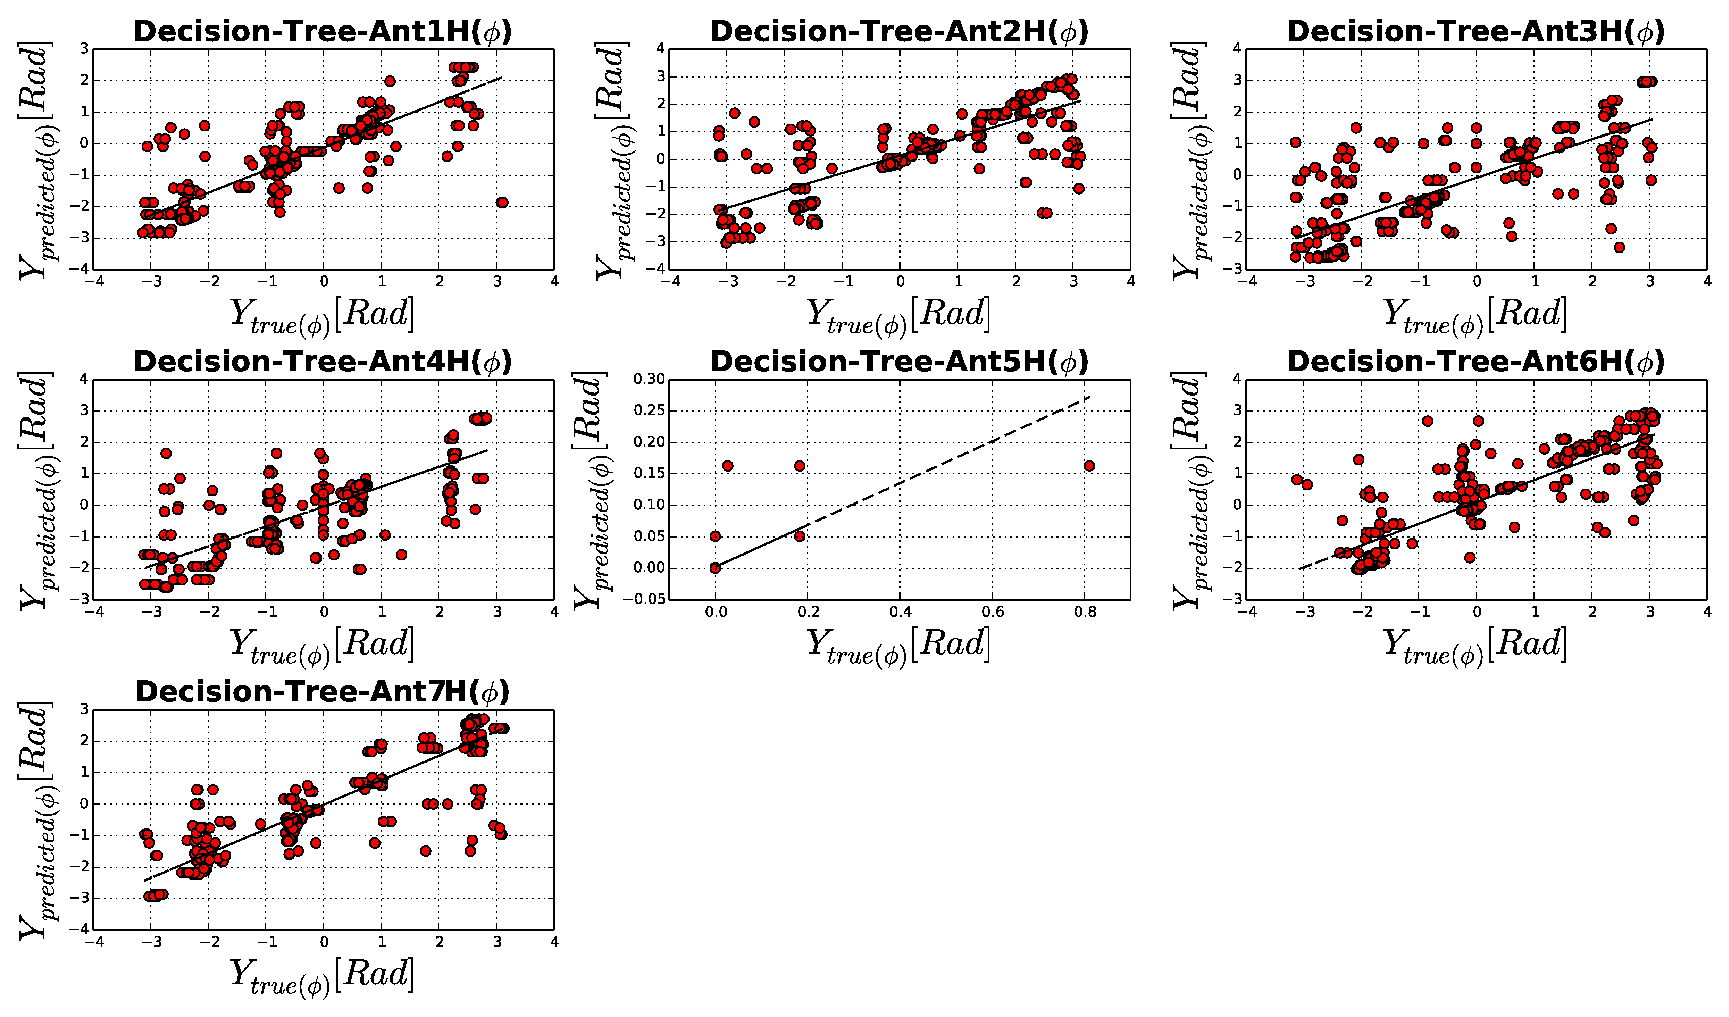
\includegraphics[width=\textwidth]{images/Decision-TreeHphase.eps} 
        \caption{Phase gain solutions for H-polarization}
         \label{A}
    \end{subfigure}
    
      \begin{subfigure}[t]{0.52\textheight}
       
        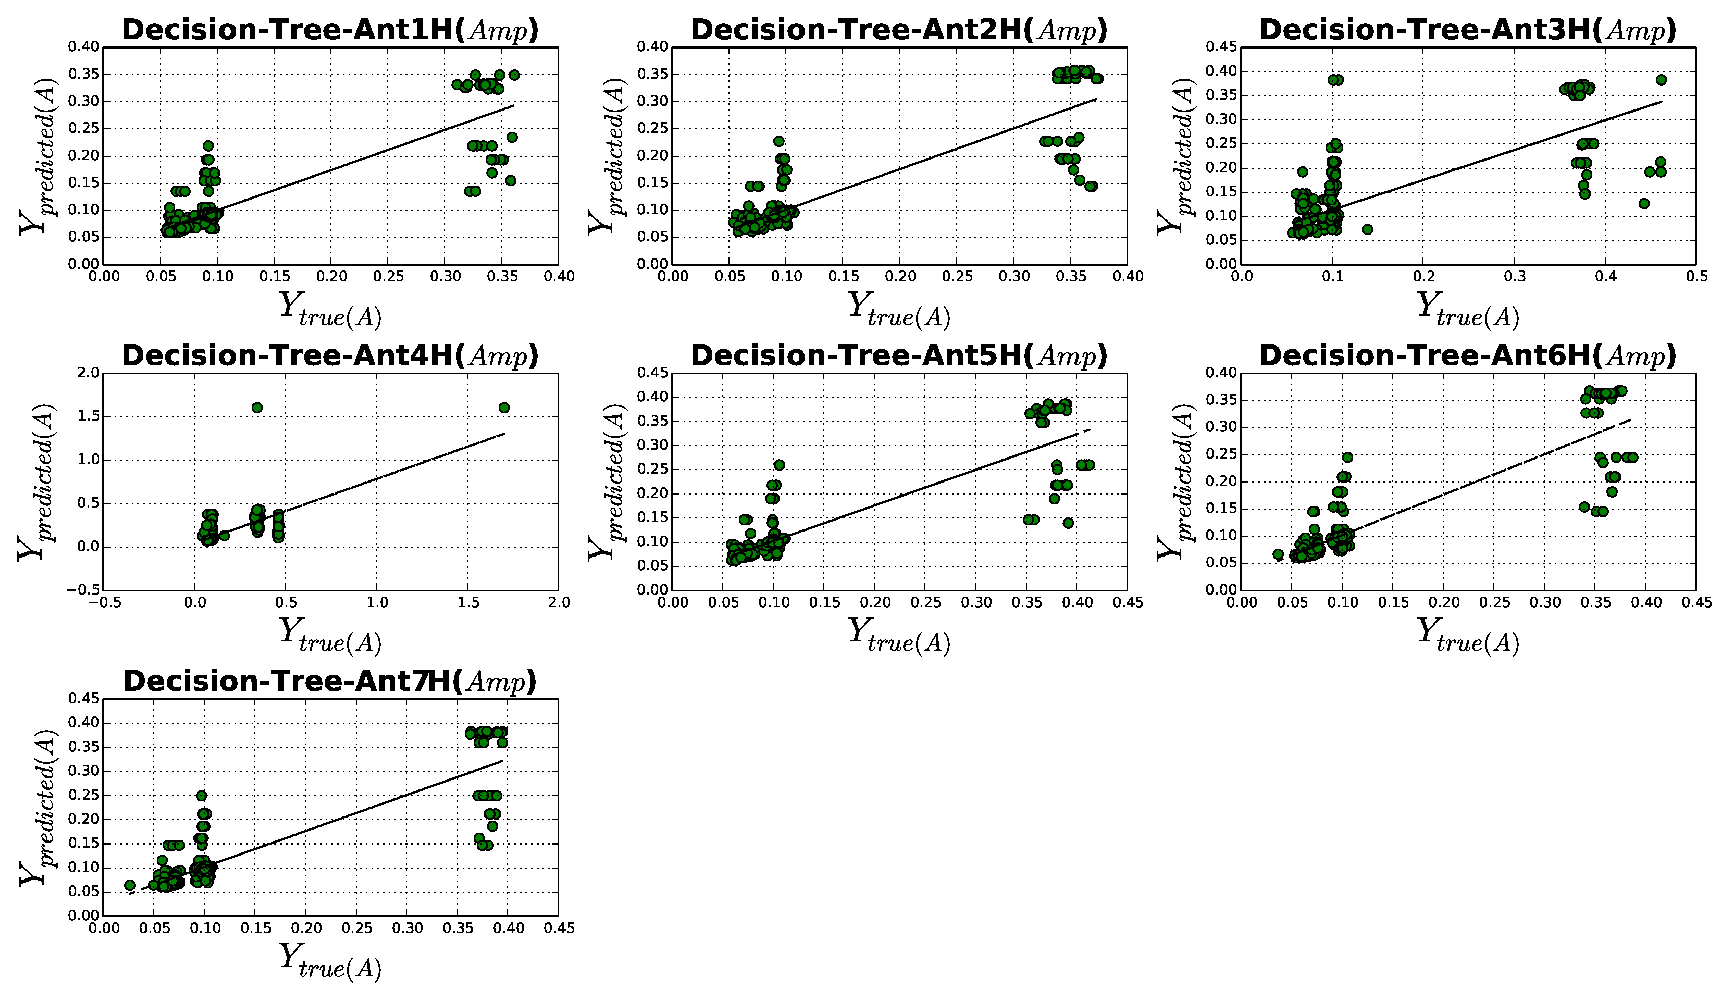
\includegraphics[width=\textwidth]{images/Decision-TreeHamp.eps} 
        \caption{Amplitude gain solutions for H-polarization.}
         \label{B}
    \end{subfigure}
    \caption{Results obtained from the decision tree learning algorithm with randomized search optimization algorithm. (\subref{A}) and (\subref{B})are the predicted gain solutions $\textbf{Y}_\mathrm{predicted}$ by the decision tree vs the true gain solutions $\textbf{Y}_\mathrm{true}$ (CASA) for H-polarization. We observe that the decision tree algorithm is performing badly in predicting the H-polarization amplitude and phase gain solutions}
 \label{BB}
    \end{figure}
  
\begin{figure}[H]
   \centering
    \begin{subfigure}[t]{0.52\textheight}
        
        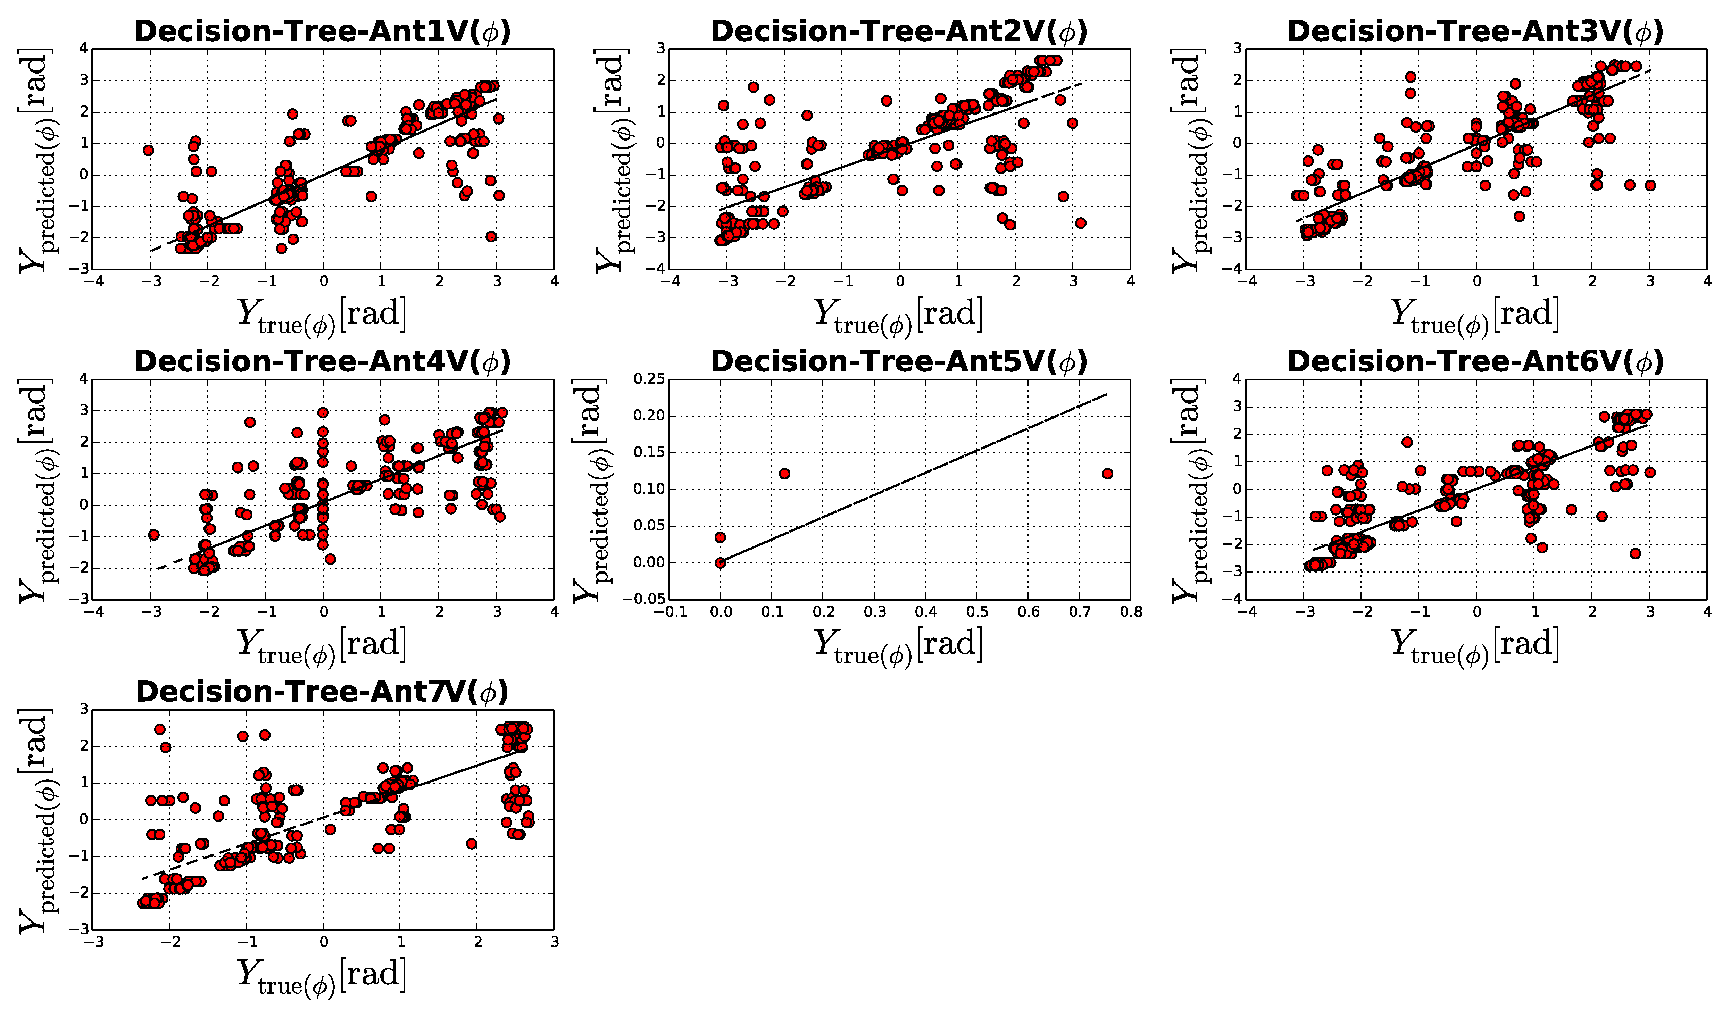
\includegraphics[width=\textwidth]{images/Decision-TreeVphase.eps} 
        \caption{Phase gain solutions for V-polarization}
         \label{A1}
    \end{subfigure}
    
      \begin{subfigure}[t]{0.52\textheight}
       
        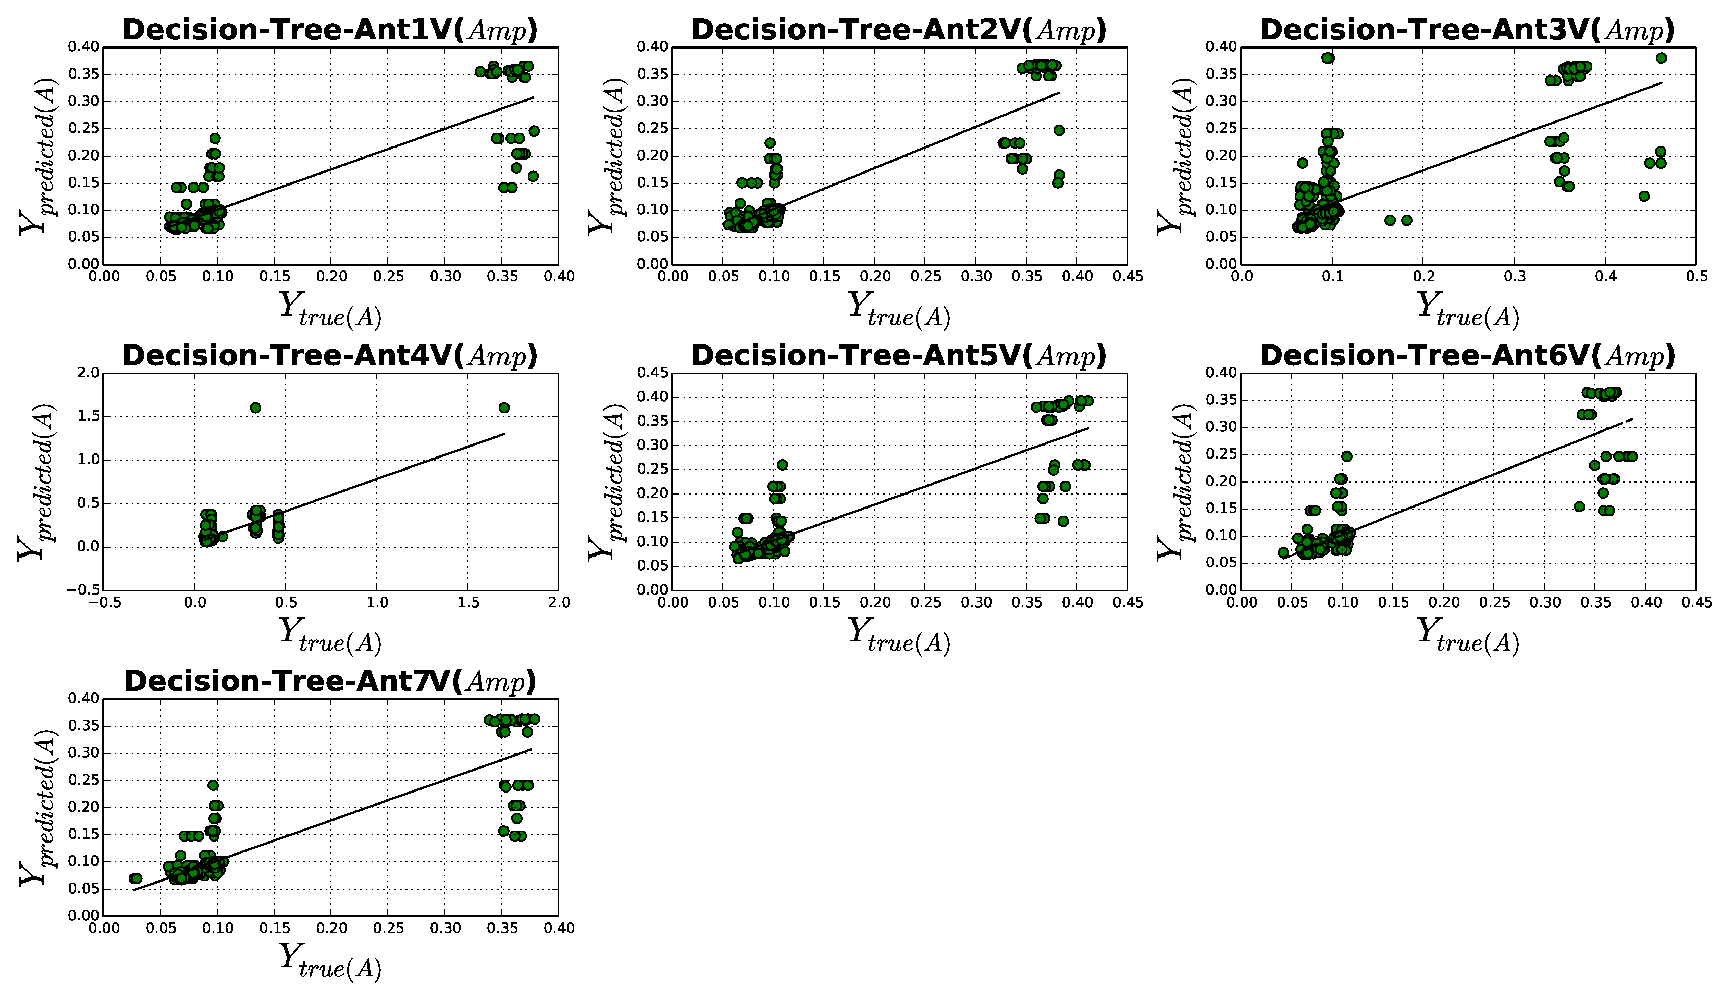
\includegraphics[width=\textwidth]{images/Decision-TreeVamp.eps} 
        \caption{Amplitude gain solutions for V-polarization} 
        \label{B1}
    \end{subfigure}
    \caption{Results obtained from the decision tree learning algorithm with randomized search optimization algorithm. (\subref{A1}) and (\subref{B1}) are the predicted gain solutions $\textbf{Y}_\mathrm{predicted}$ by the decision tree vs the true gain solutions $\textbf{Y}_\mathrm{true}$ (CASA) for V-polarization. Similar to H-polarization above, the decision tree algorithm is failing to predict V-polarization amplitude and phase gain solutions.}
 \label{BB1}
    \end{figure}
    
\begin{table}[H]
\label{T:equipos}
\begin{center}
\scalebox{0.7}{
\begin{tabular}{| c | c | c | c | c |}
\hline
Antenna & \multicolumn{4}{ c |}{\textbf{Decision tree phase}}  \\ 
\cline{2-5}
&Rmse & Rmae & R2score &Explained $\sigma^2$\\
\hline
Uniform average-H &0.573 & 0.417 & 0.820   & 0.821 \\ 
Uniform average-V &0.435 & 0.367 & 0.879    & 0. 879\\ \hline
 & \multicolumn{4}{ c |}{\textbf{Decision tree amplitude}}  \\ 
\cline{1-5}
\hline
Uniform average-H &0.043 & 0.109 & 0.835   & 0.835 \\ 
Uniform average-V &0.043 & 0.109 & 0.831    & 0.831\\\hline
\end{tabular}}
\end{center}
\caption{The table shows the performance of the decision tree algorithm in predicting the amplitude and phase gain solutions for both H and V polarizations as shown in Figures \ref{BB} and \ref{BB1}. The values shown represent uniform average of all KAT-7 antennas, i.e., all output measures are averaged with uniform weight. Most of the predictions scatter away from the ideal truth values.}
\end{table}

\subsection{Random forest training}
\begin{figure}[H]
   \centering
    \begin{subfigure}[t]{0.52\textheight}
        
        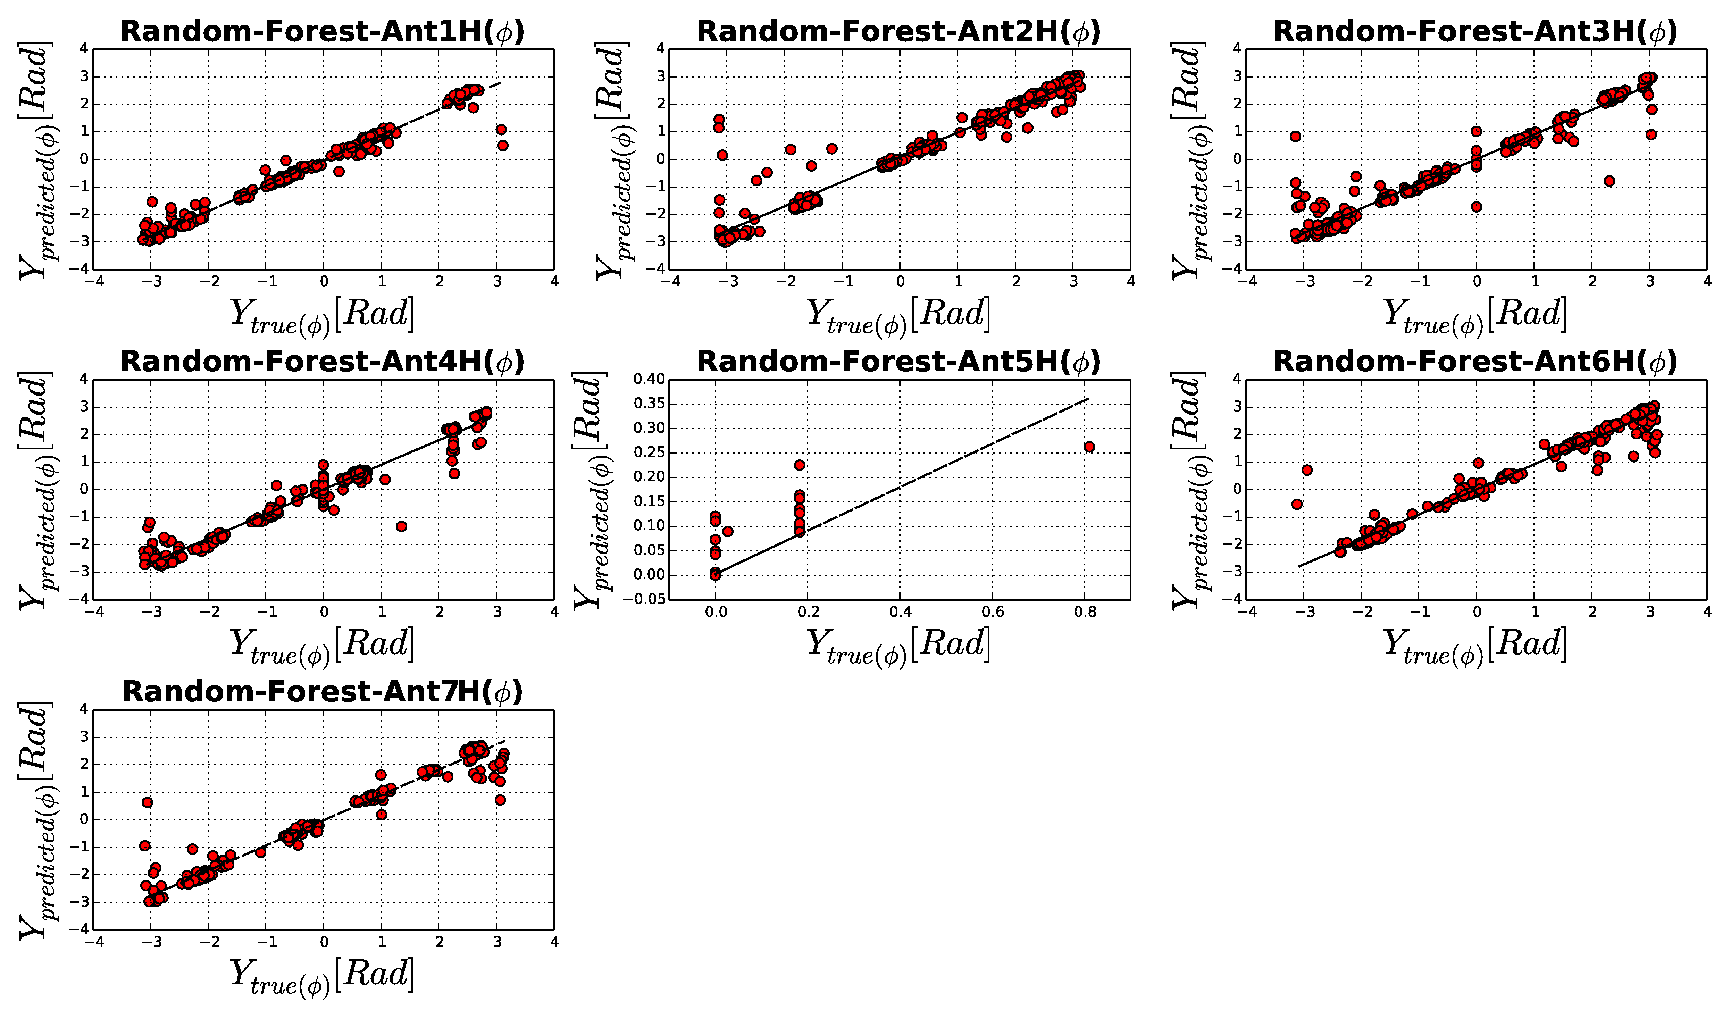
\includegraphics[width=\textwidth]{images/Random-ForestHphase.eps} 
        \caption{Phase gain solutions for H-polarization} \label{A2}
    \end{subfigure}
    
      \begin{subfigure}[t]{0.52\textheight}
       
        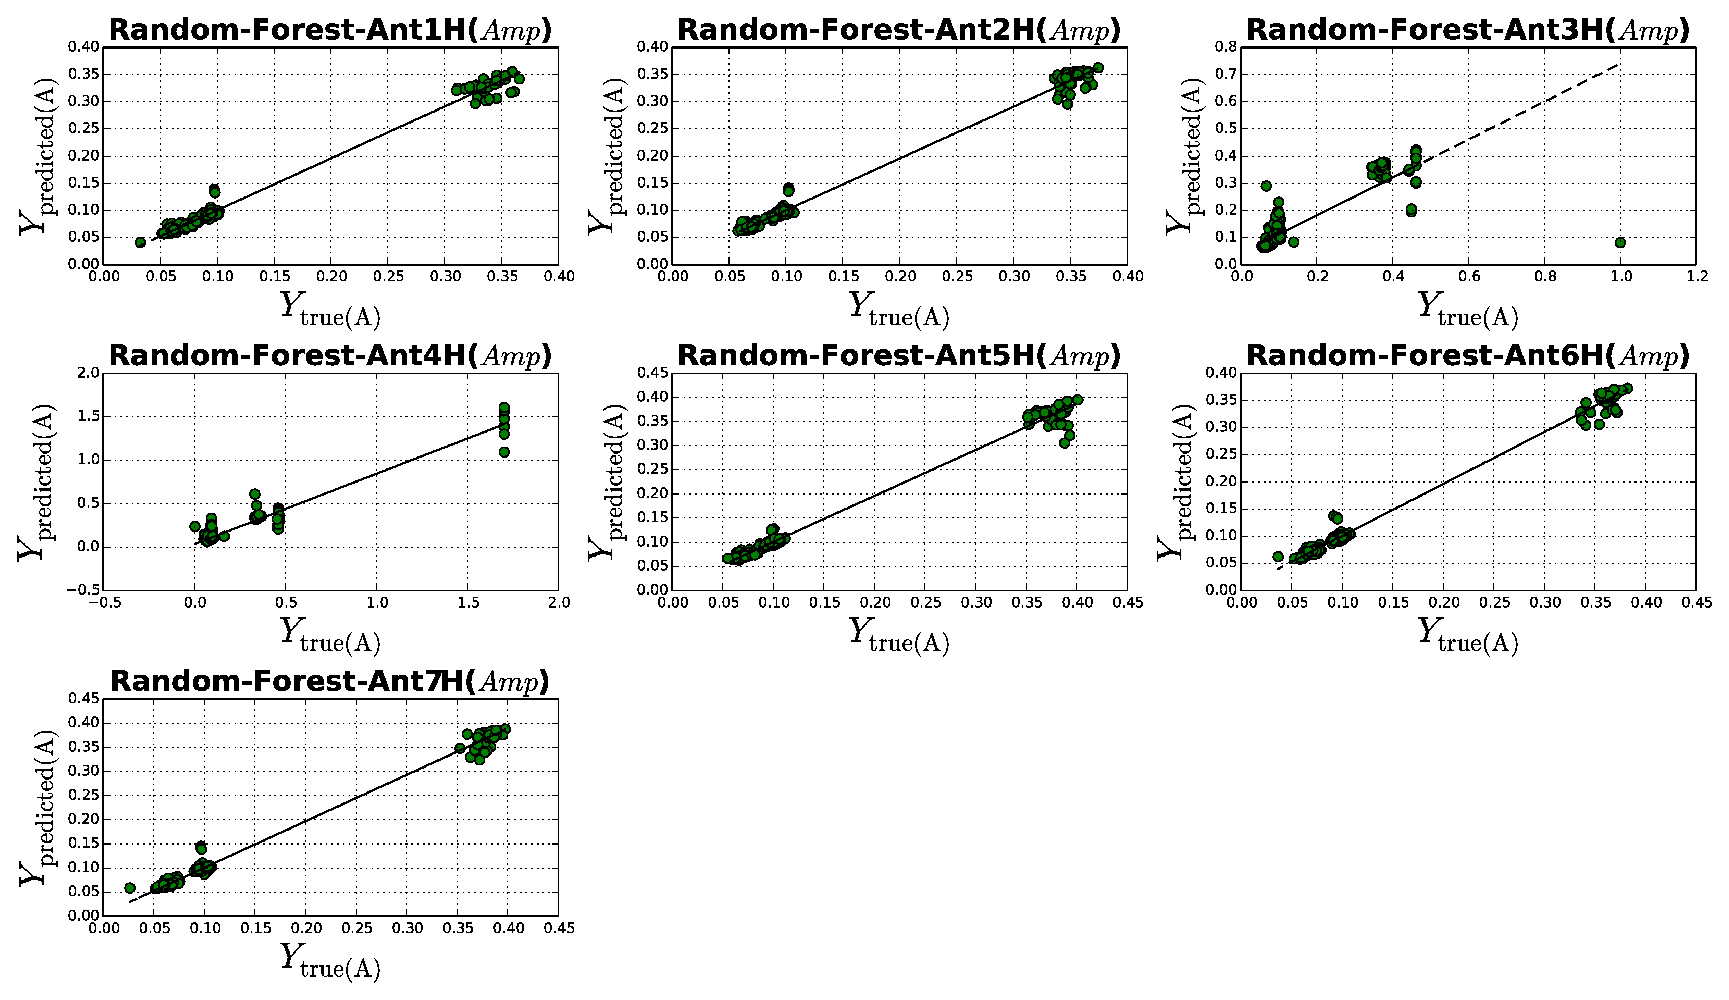
\includegraphics[width=\textwidth]{images/Random-ForestHamp.eps} 
        \caption{Amplitude gain solutions for H-polarization} \label{B2}
    \end{subfigure}
    \caption{Results obtained from the random forest learning algorithm with randomized search optimization algorithm. Figures (\subref{A2}) and (\subref{B2}) are the predicted gain solutions $\textbf{Y}_\mathrm{predicted}$ by the random forest vs the true gain solutions $\textbf{Y}_\mathrm{true}$ (CASA) for H-polarization. We observe that the random forest algorithm is performing better in predicting the H-polarization amplitude and phase gain solutions with few outlier points.}
    \label{BB2}
    \end{figure}
    
\begin{figure}[H]
   \centering
    \begin{subfigure}[t]{0.52\textheight}
        
        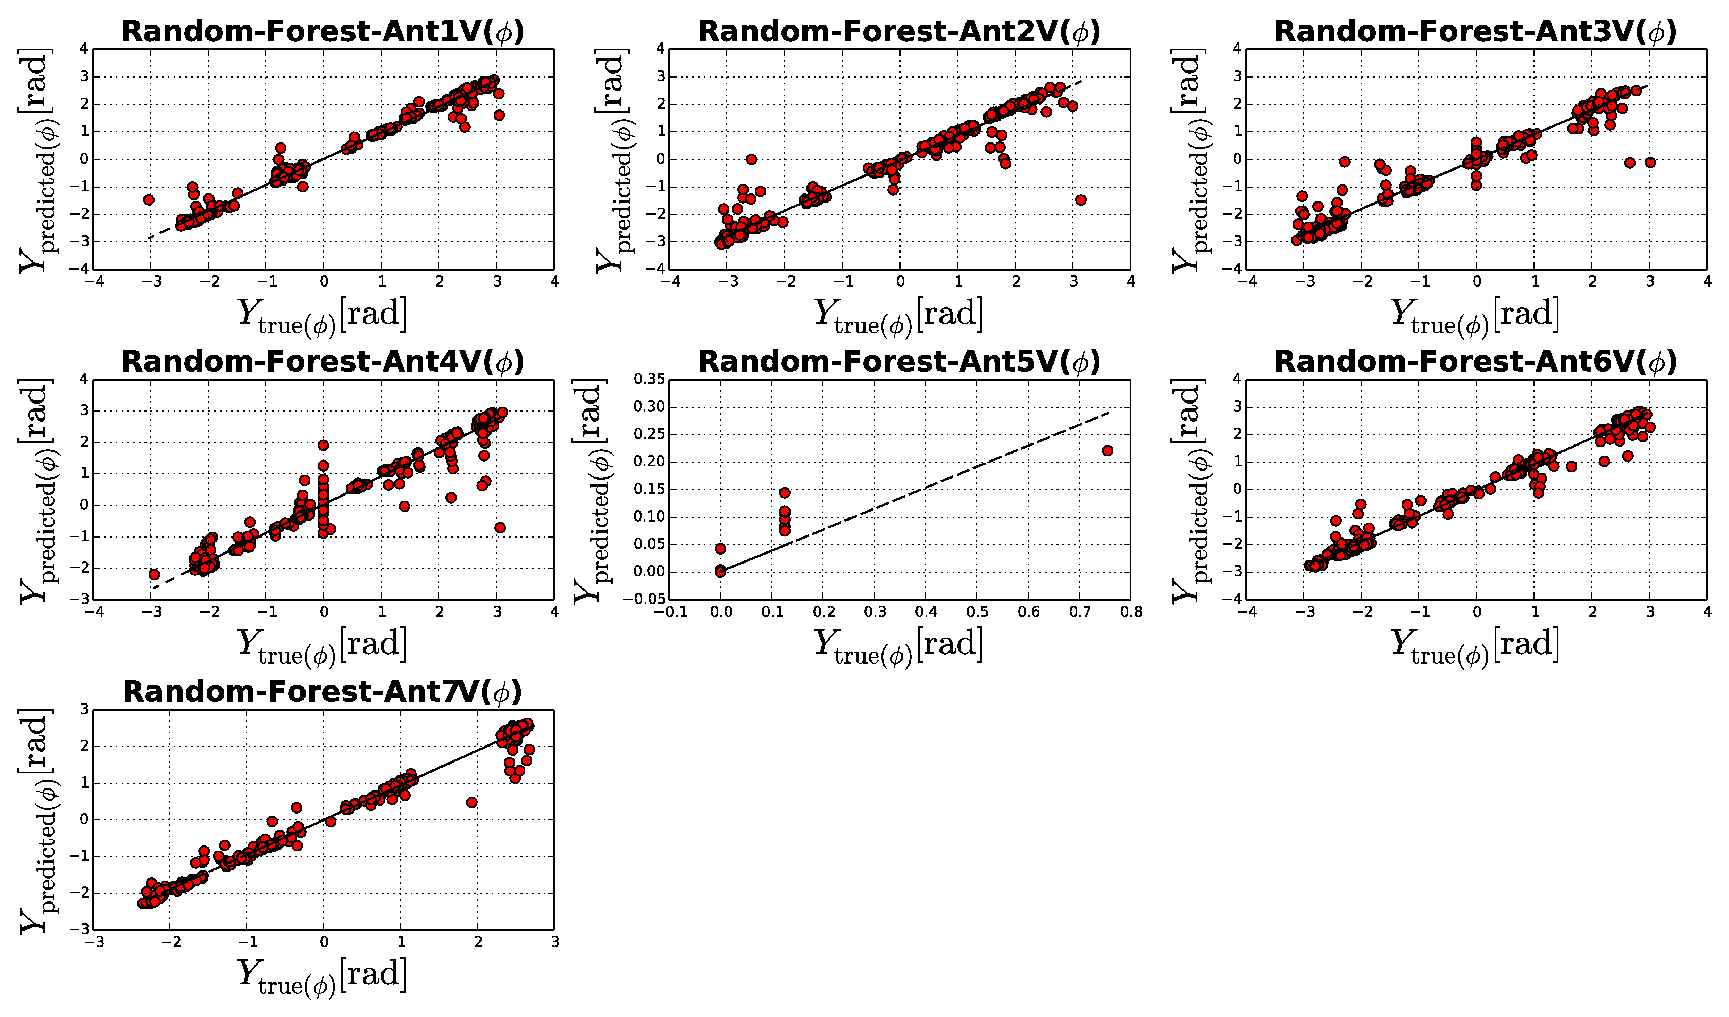
\includegraphics[width=\textwidth]{images/Random-ForestVphase.eps} 
        \caption{Phase gain solutions for V-polarization} \label{A3}
    \end{subfigure}
    
      \begin{subfigure}[t]{0.52\textheight}
       
        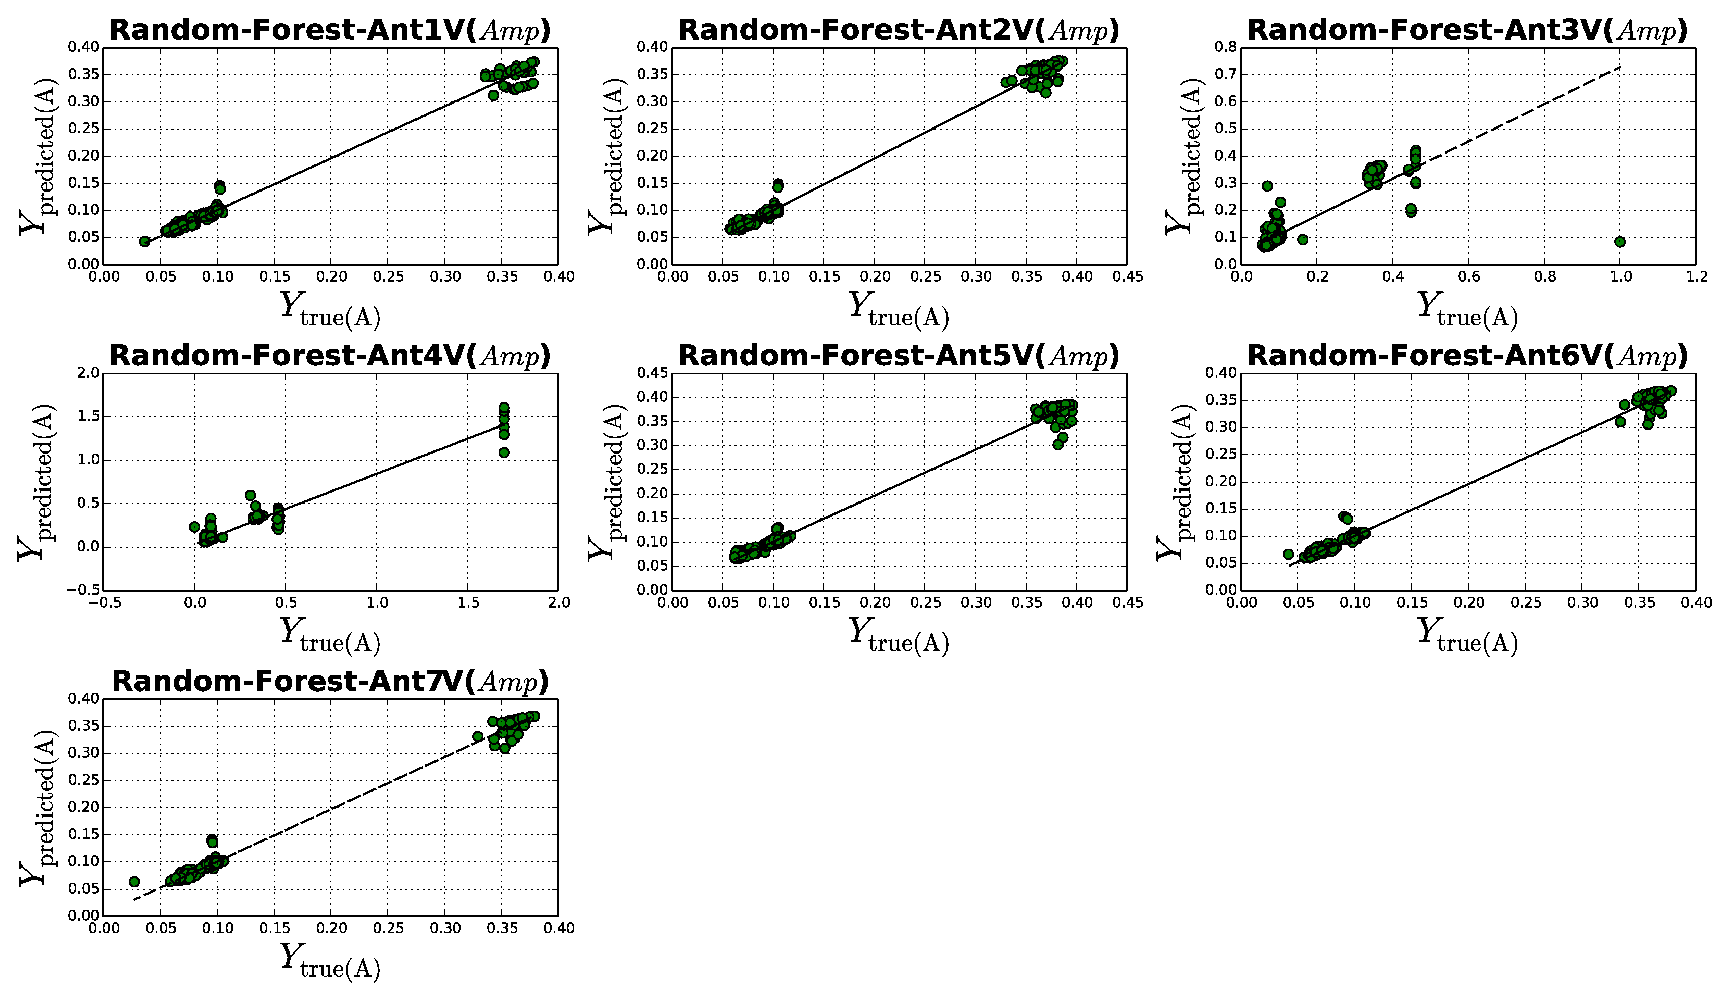
\includegraphics[width=\textwidth]{images/Random-ForestVamp.eps} 
        \caption{Amplitude gain solutions for V-polarization} \label{B3}
    \end{subfigure}
    \caption{Results obtained from the random forest learning algorithm with randomized search optimization algorithm. (\subref{A3}) and (\subref{B3}) are the predicted phase gain solutions $\textbf{Y}_\mathrm{predicted}$ by the random forest vs the true gain solutions $\textbf{Y}_\mathrm{true}$ (CASA) for V polarization. We observe that the random forest is performing better in predicting the V-polarization amplitude and phase gain solutions with few outlier points. }
    \label{BBB2}
    \end{figure} 
   
\begin{table}[H]
\begin{center}
\scalebox{0.7}{
\begin{tabular}{| c | c | c | c | c |}
\hline
Antenna & \multicolumn{4}{ c |}{\textbf{Random forest phase}}  \\ 
\cline{2-5}
& Rmse & Rmae & R2score & Explained $\sigma^2$\\
\hline
 Uniform average-H &0.368 & 0.352 & 0.912   & 0.912 \\ 
Uniform average-V &0.256 & 0.311 & 0.939   & 0.939\\ \hline
 & \multicolumn{4}{ c |}{\textbf{Random forest amplitude}}  \\ 
\cline{1-5}
\hline
Uniform average-H &0.028 & 0.087 & 0.918   & 0.919 \\ 
Uniform average-V &0.028 & 0.088 & 0.916    & 0.917\\ \hline

\end{tabular}}
\end{center}
\caption{The table shows the performance of the random forest algorithm in predicting the amplitude and phase  gain solutions for both H and V polarizations as shown in Figures \ref{BB2} and \ref{BBB2}. The values shown represent the uniform average of all KAT-7 antennas, i.e., all output measures are averaged with uniform weight. We observe that most of the predictions stay near the ideal truth values with rmse \ref{MSE} and rmae \ref{MAE}  $\approx <$ 0.5, $R^2$ \ref{R2score} and explained variance $V$ \ref{ExV} converging to 1.}
\end{table}

\subsection{K-nearest neighbor training}
\begin{figure}[H]
   \centering
    \begin{subfigure}[t]{0.52\textheight}
        
        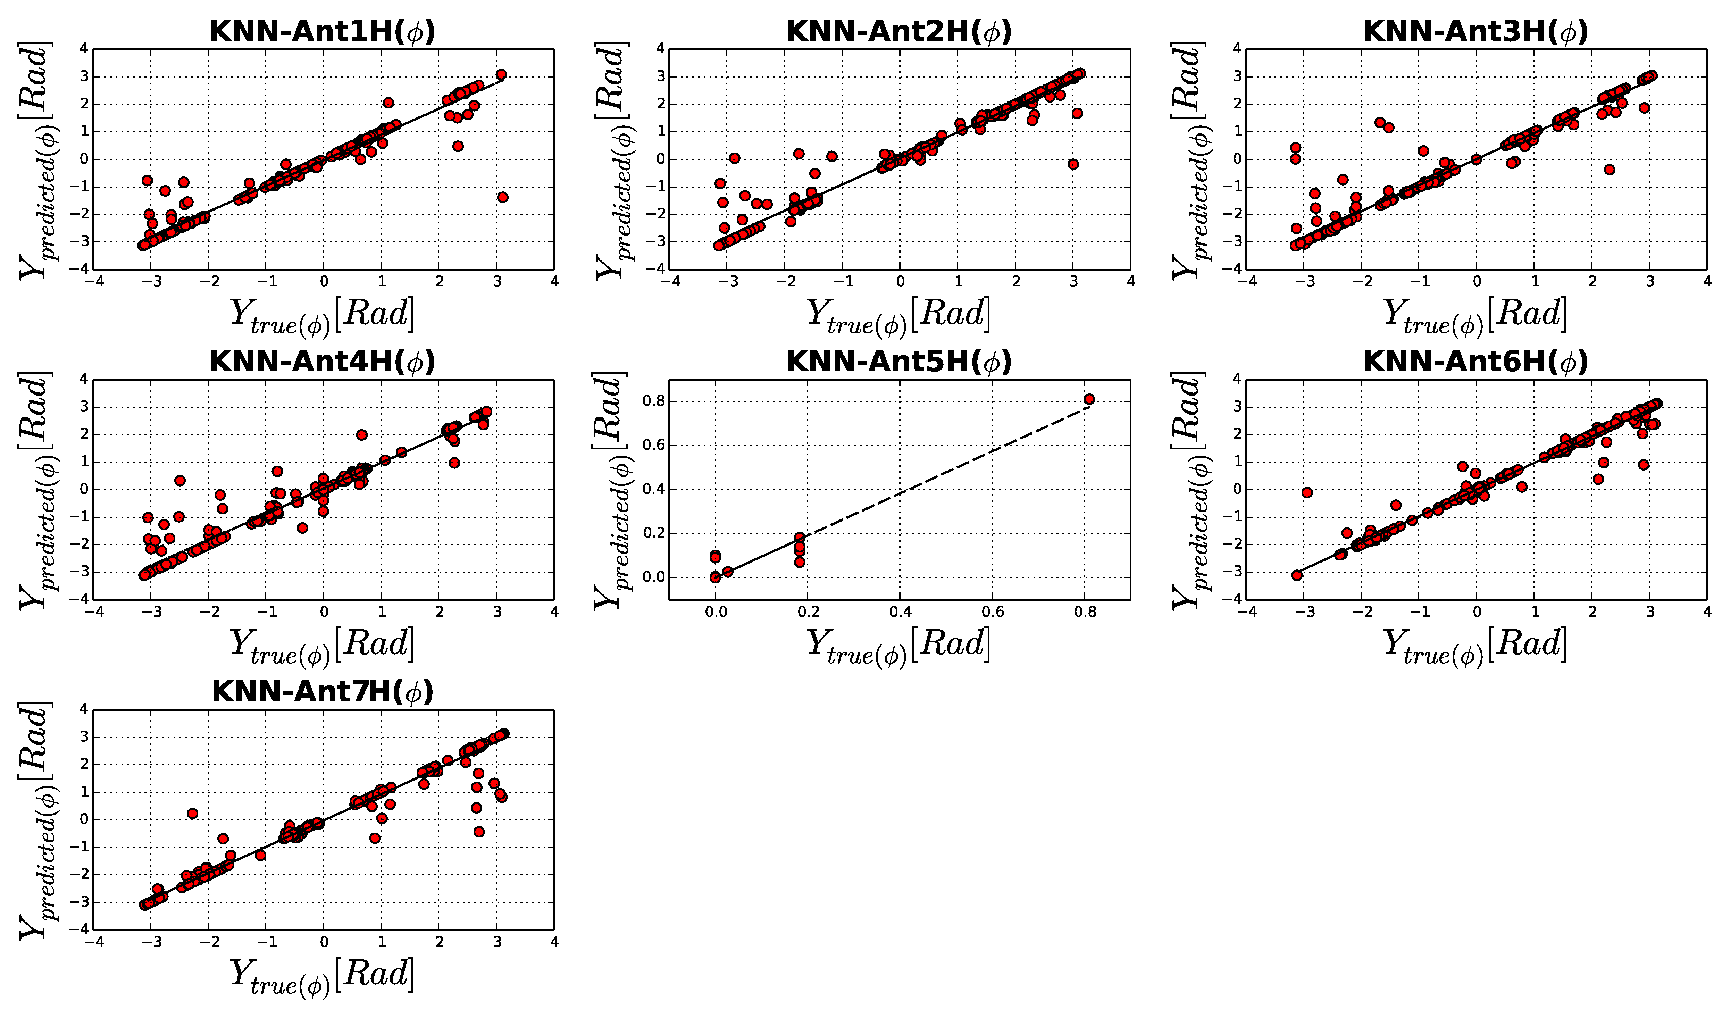
\includegraphics[width=\textwidth]{images/KNNHphase.eps} 
        \caption{Phase gain solutions for H-polarization} \label{A4}
    \end{subfigure}
    
      \begin{subfigure}[t]{0.52\textheight}
       
        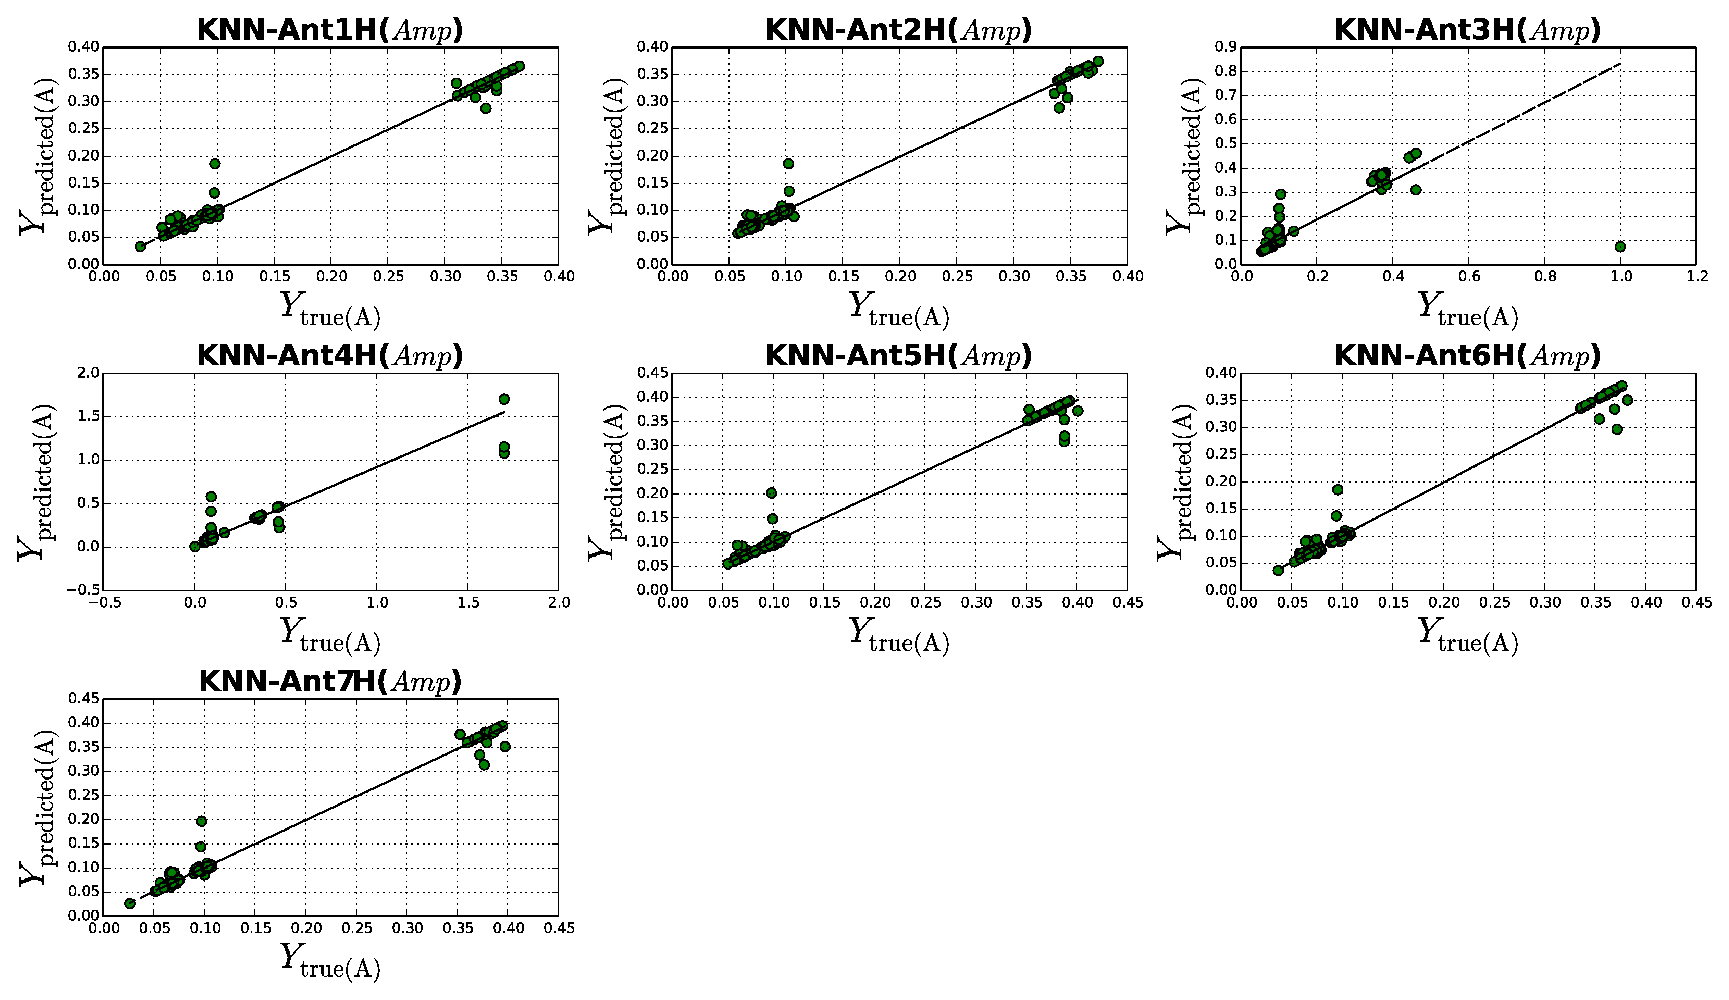
\includegraphics[width=\textwidth]{images/KNNHamp.eps} 
        \caption{Amplitude gain solutions for H-polarization} \label{B4}
    \end{subfigure}
    \caption{Results obtained from the K-nearest neighbor learning algorithm with randomized search optimization algorithm. (\subref{A4}) and (\subref{B4}) are the predicted gain solutions $\textbf{Y}_\mathrm{predicted}$ by the K-nearest neighbor vs the true gain solutions $\textbf{Y}_\mathrm{true}$ (CASA) for H-polarization. We observe that the K-nearest neighbor is performing better in predicting the H-polarization amplitude and phase gain solutions with few outlier points.}
    \label{BB4}
    \end{figure}
    
\begin{figure}[H]
   \centering
    \begin{subfigure}[t]{0.52\textheight}
        
        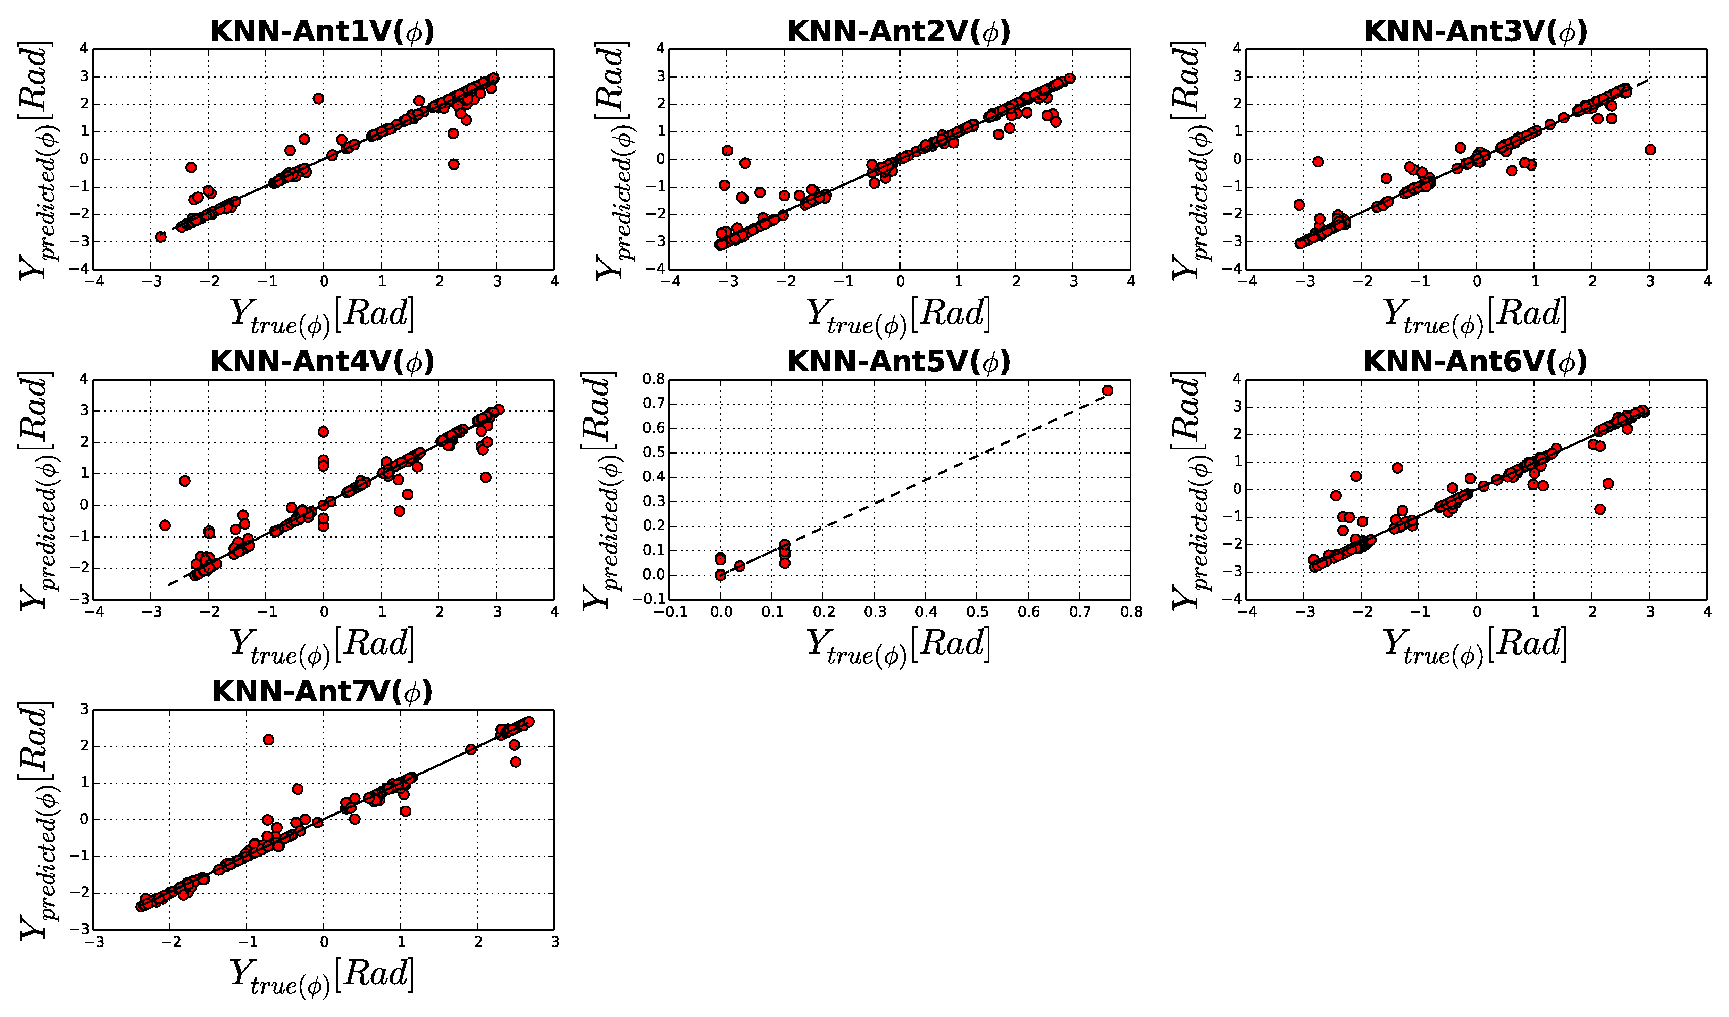
\includegraphics[width=\textwidth]{images/KNNVphase.eps} 
        \caption{Phase gain solutions for V-polarization} \label{A5}
    \end{subfigure}
    
      \begin{subfigure}[t]{0.52\textheight}
       
        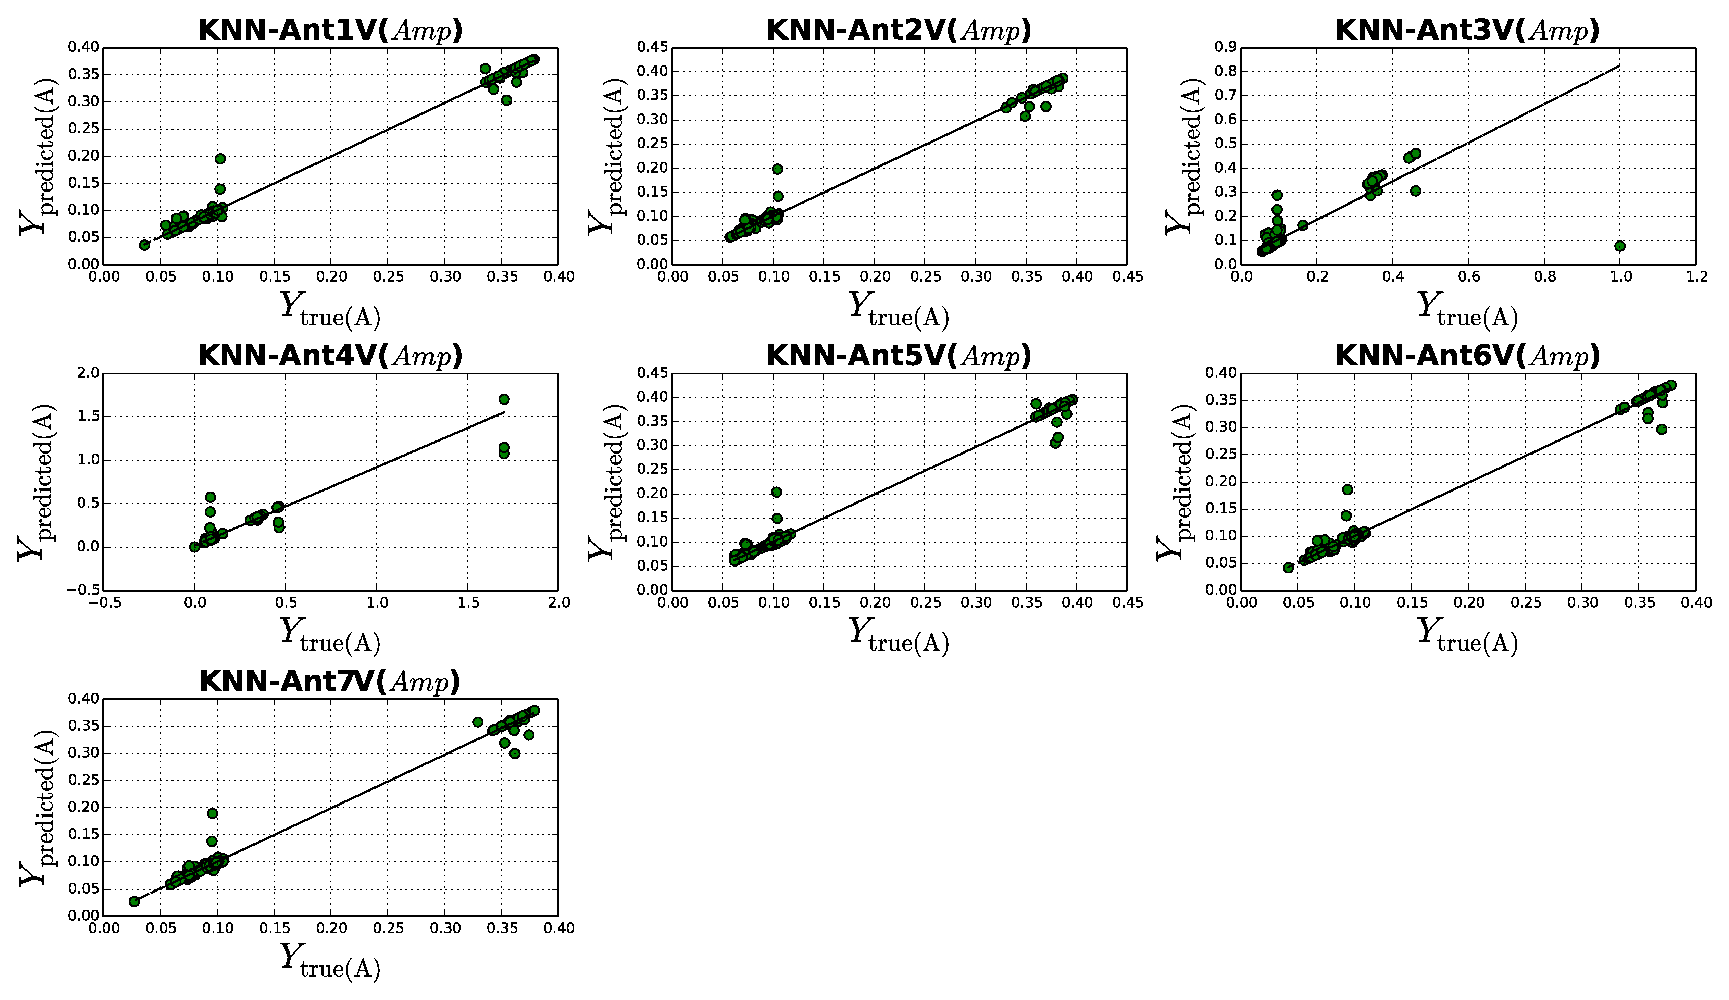
\includegraphics[width=\textwidth]{images/KNNVamp.eps} 
        \caption{Amplitude gain solutions for V-polarization} \label{B5}
    \end{subfigure}
    \caption{Results obtained from the K-nearest neighbor learning algorithm with randomized search optimization algorithm. (\subref{A5}) and (\subref{B5}) are the predicted phase gain solutions $\textbf{Y}_\mathrm{predicted}$ by the K-nearest neighbor vs the true phase gain solutions $\textbf{Y}_\mathrm{true}$ (CASA) for V-polarization. We observe that the K-nearest neighbor is performing better in predicting the V-polarization amplitude and phase gain solutions with few outlier points. }
    \label{BBB4}
    \end{figure} 
   

\begin{table}[H]
\label{T:equipos}
\begin{center}
\scalebox{0.7}{
\begin{tabular}{| c | c | c | c | c |}
\hline
Antenna & \multicolumn{4}{ c |}{\textbf{KNN phase}}  \\ 
\cline{2-5}
& Rmse &Rmae &R2score&Explained$\sigma^2$\\
\hline

 Uniform average-H &0.352 & 0.258 & 0.945    & 0.945 \\ 
Uniform average-V &0.291 & 0.239 & 0.961    & 0. 961\\ \hline
 & \multicolumn{4}{ c |}{\textbf{KNN amplitude}}  \\ 
\cline{1-5}
\hline
 Uniform average-H &0.352 & 0.258 & 0.945    & 0.945 \\ 
Uniform average-V &0.291 & 0.239 & 0.961    & 0. 961\\ \hline
\end{tabular}}
\end{center}
\caption{The table shows the performance of the K-nearest neighbor algorithm in predicting the amplitude and phase gain solutions for both H and V polarizations as shown in Figure \ref{BB4} and \ref{BBB4}. The values shown represent the uniform average of all KAT-7 antennas, i.e., all output measures are averaged with uniform weight. Most of the predictions stay near the ideal truth values with RMSE \ref{MSE} and rmae \ref{MAE}  $\approx <$ 0.5, $R^2$ \ref{R2score} and explained variance $V$ \ref{ExV} are converging to 1.}
\end{table}


\subsection{Extremely randomized tree training}

\begin{figure}[H]
   \centering
    \begin{subfigure}[t]{0.52\textheight}
        
        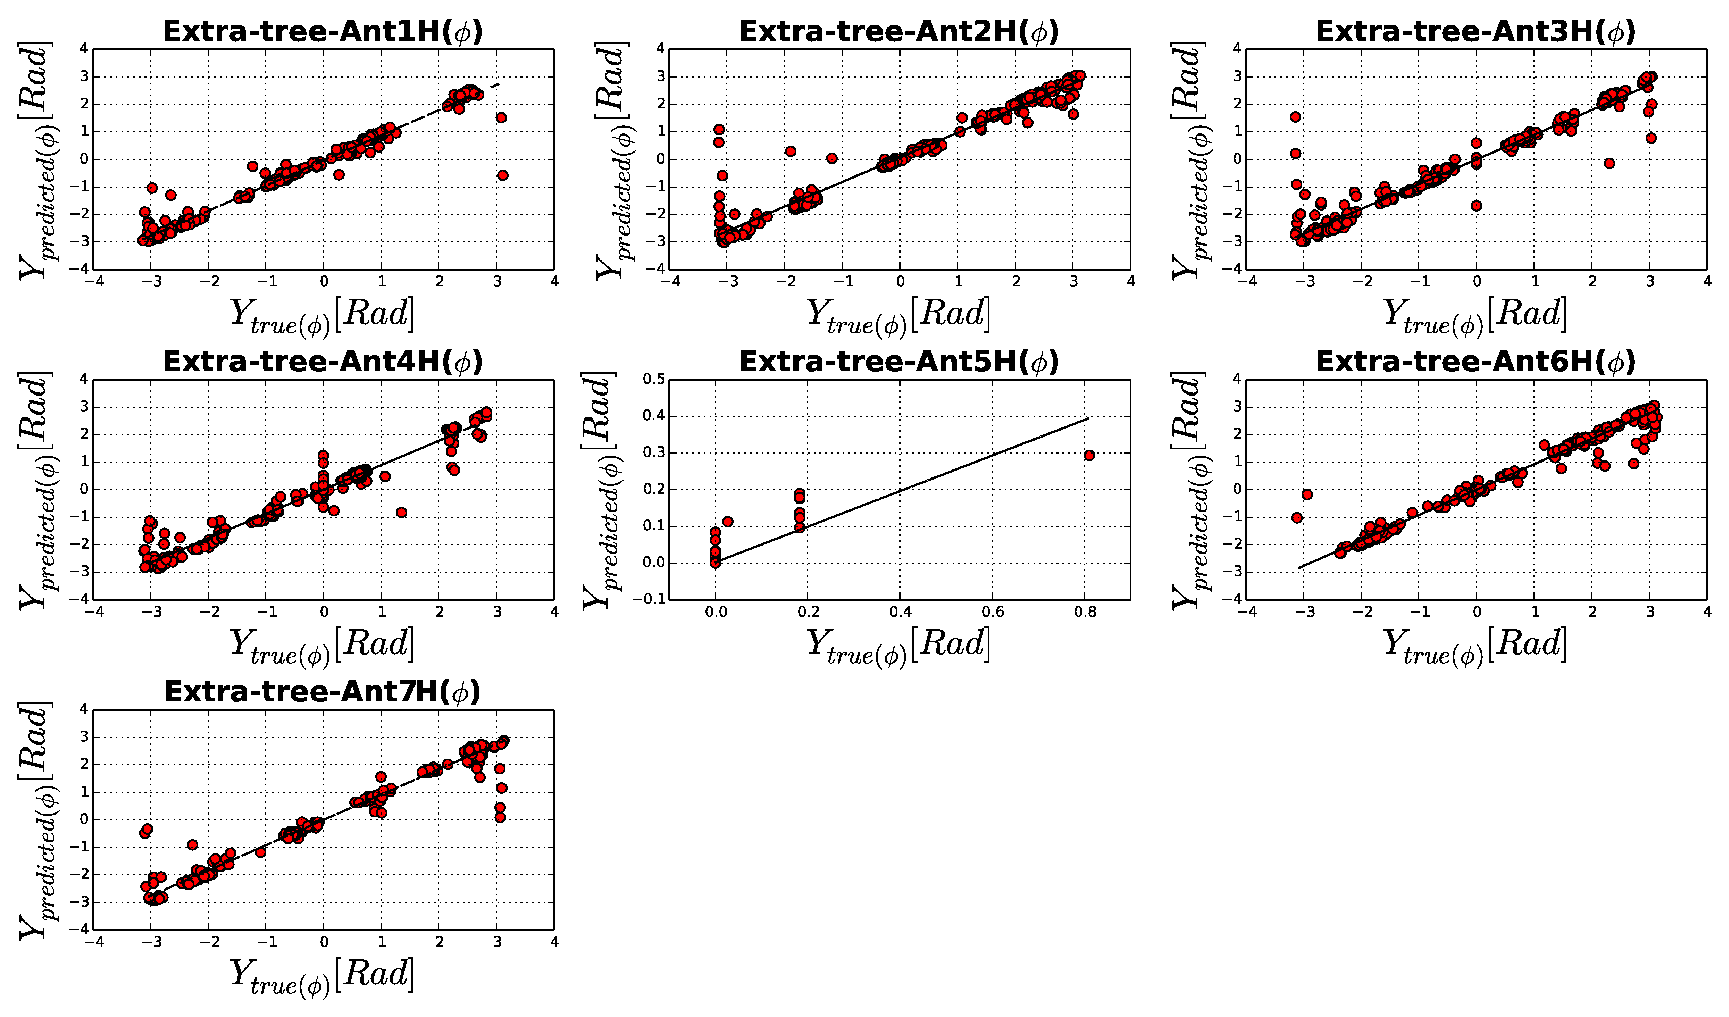
\includegraphics[width=\textwidth]{images/Extra-treeHphase.eps} 
        \caption{Phase gain solutions for H-polarization} \label{A6}
    \end{subfigure}
    
      \begin{subfigure}[t]{0.52\textheight}
       
        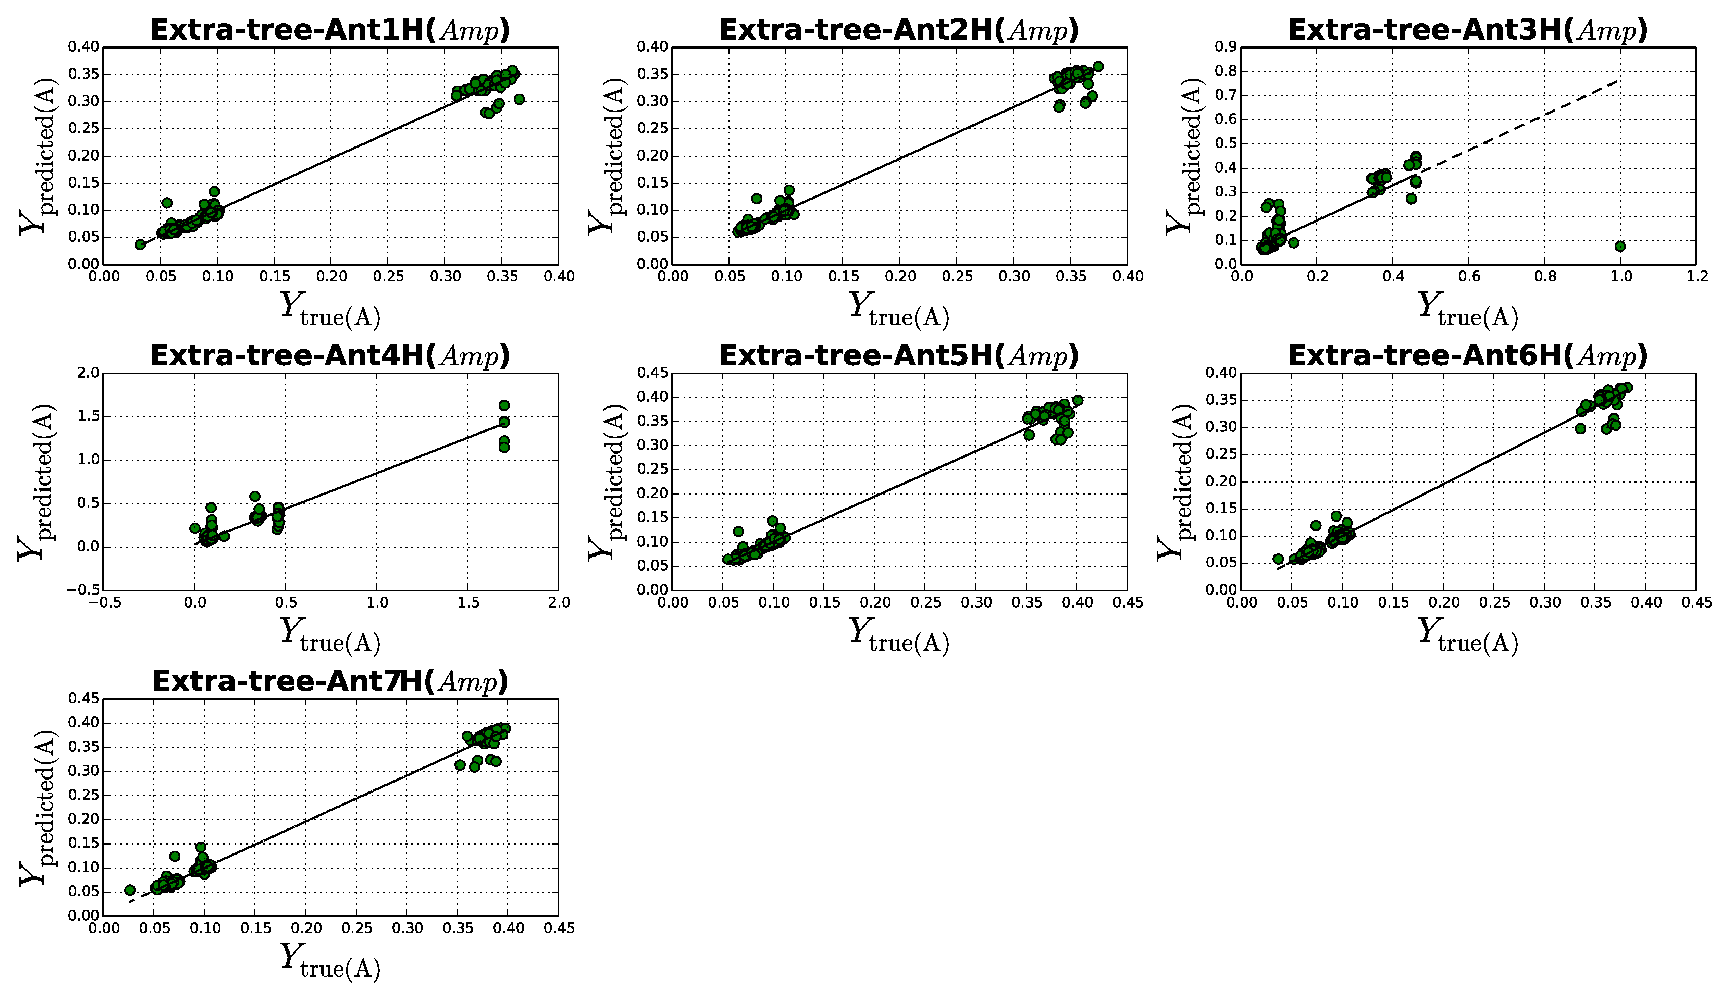
\includegraphics[width=\textwidth]{images/Extra-treeHamp.eps} 
        \caption{Amplitude gain solutions for H-polarization} \label{B6}
    \end{subfigure}
    \caption{Results obtained from the extremely randomized tree learning algorithm with randomized search optimization algorithm. (\subref{A6}) and (\subref{B6}) are the predicted gain solutions $\textbf{Y}_\mathrm{predicted}$ by the extremely randomized tree  vs the true gain solutions $\textbf{Y}_\mathrm{true}$ (CASA) for H-polarization. We observe that the extremely randomized tree is performing better in predicting the H-polarization amplitude and phase gain solutions with few outlier points.}
    \label{BB7}
    \end{figure}
    
\begin{figure}[H]
   \centering
    \begin{subfigure}[t]{0.52\textheight}
        
        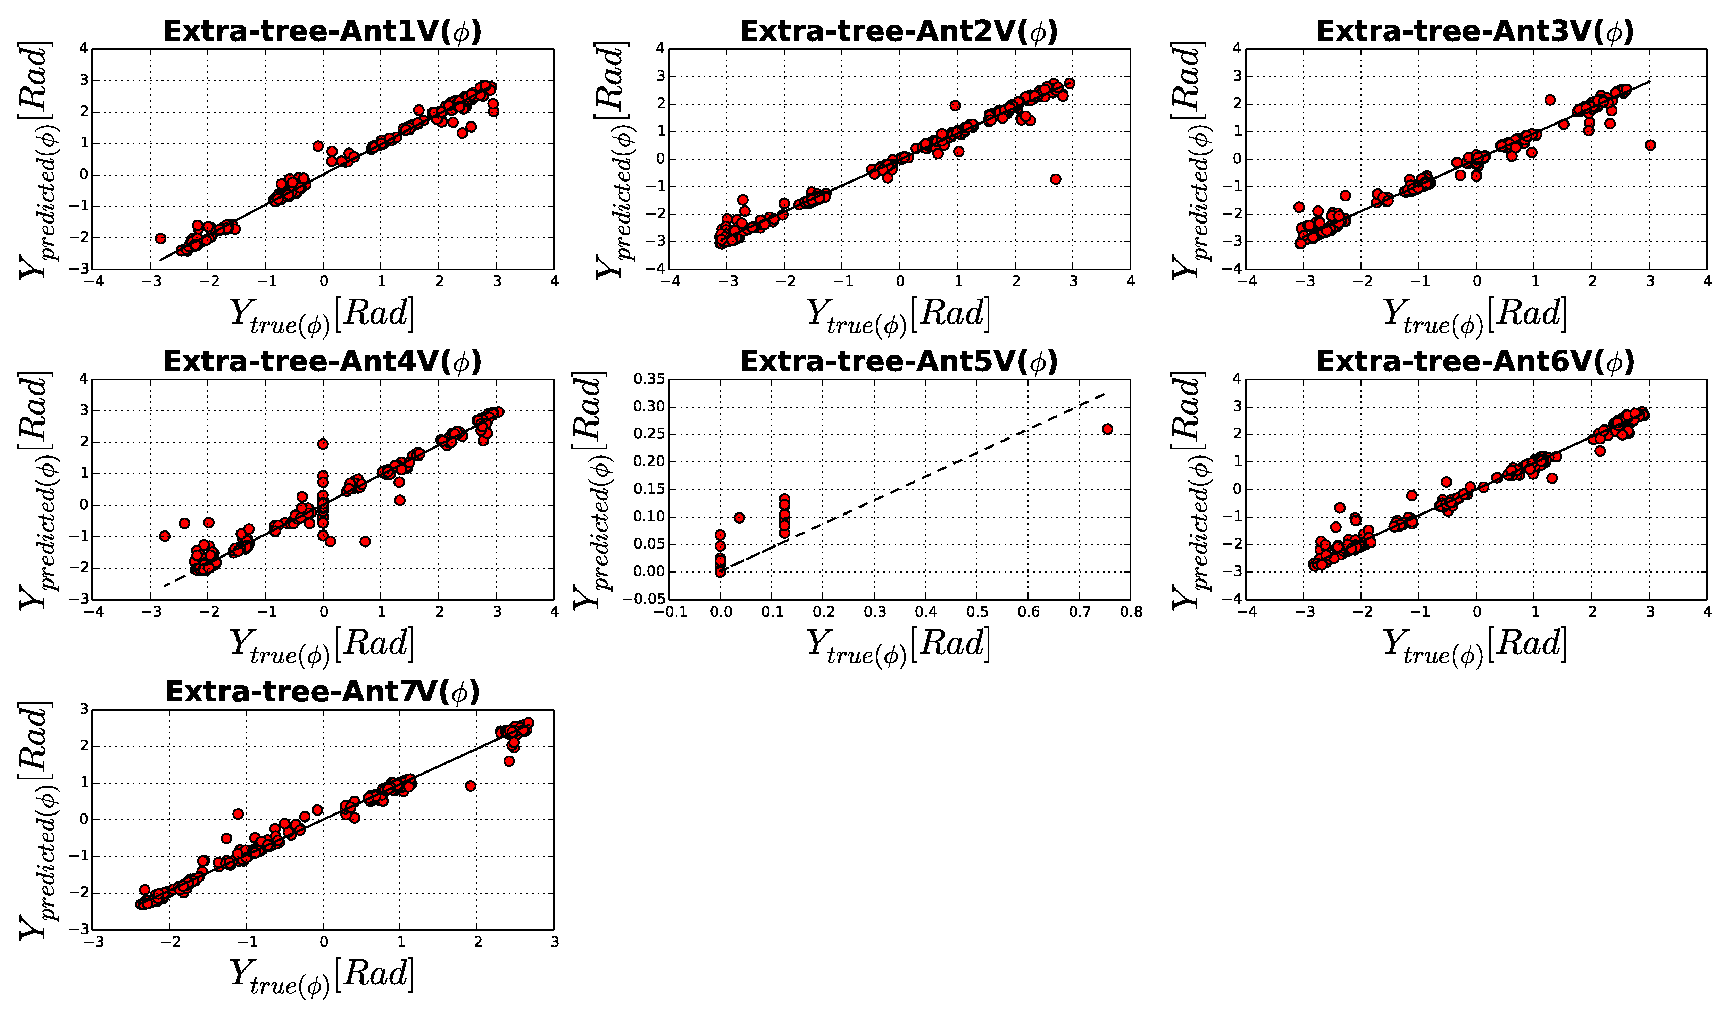
\includegraphics[width=\textwidth]{images/Extra-treeVphase.eps} 
        \caption{Phase gain solutions for V-polarization} \label{A7}
    \end{subfigure}
    
      \begin{subfigure}[t]{0.52\textheight}
       
        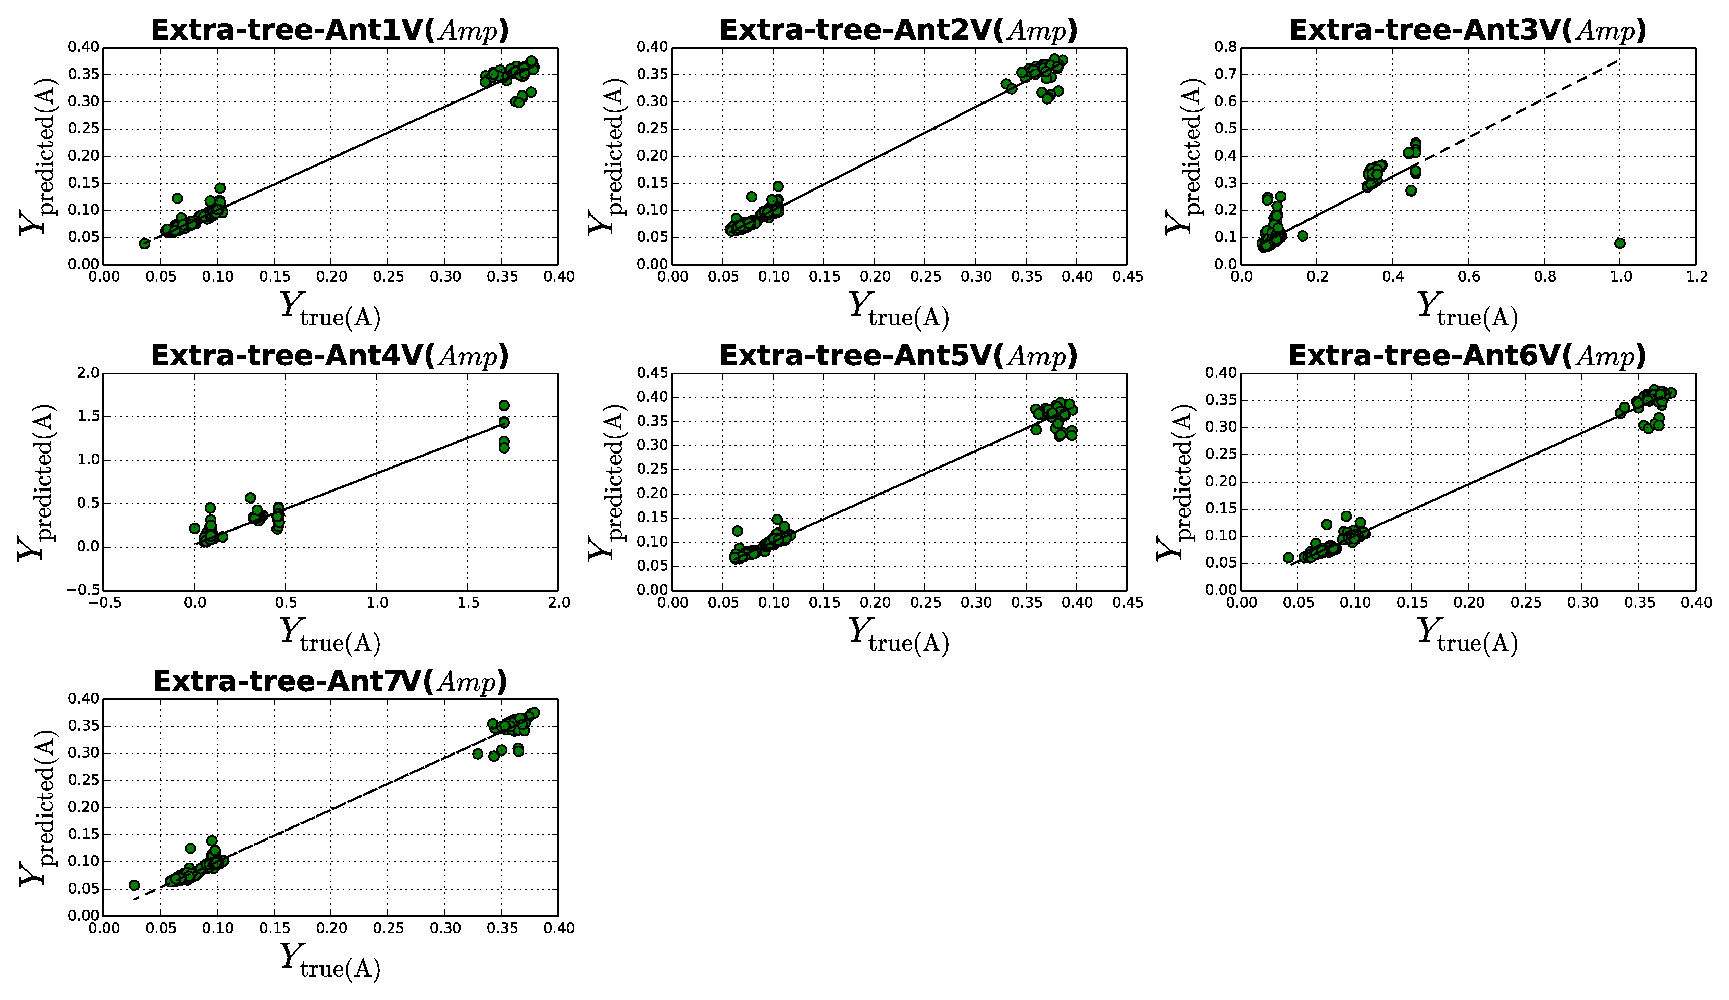
\includegraphics[width=\textwidth]{images/Extra-treeVamp.eps} 
        \caption{Amplitude gain solutions for V-polarization} \label{B7}
    \end{subfigure}
    \caption{Results obtained from the extremely randomized tree learning algorithm with randomized search optimization algorithm. (\subref{A7}) and (\subref{B7}) are the predicted gain solutions $\textbf{Y}_\mathrm{predicted}$ by the learning algorithm vs the true gain solutions $\textbf{Y}_\mathrm{true}$ (CASA) for V-polarization. We observe that the extremely randomized tree is performing better in predicting the V-polarization amplitude and phase gain solutions with few outlier points. }
    \label{BBB7}
    \end{figure} 
   
\begin{table}[H]
\label{T:equipos}
\begin{center}
\scalebox{0.7}{
\begin{tabular}{| c | c | c | c | c |}
\hline
Antenna & \multicolumn{4}{ c |}{\textbf{Extremely randomized phase}}  \\ 
\cline{2-5}
& rmse & Rmae & R2score & Explained $\sigma^2$\\
\hline
 Uniform average-H &0.337 & 0.336 & 0.936    & 0.936 \\ 
Uniform average-V &0.235 & 0.301 & 0.956    & 0. 957\\ \hline
 & \multicolumn{4}{ c |}{\textbf{Extremely randomized tree  amplitude}}  \\ 
\cline{1-5}
\hline
Uniform average-H &0.027 & 0.083 & 0.925    & 0.925 \\ 
Uniform average-V &0.027 & 0.083 & 0.923    & 0.923 \\ \hline
\end{tabular}}
\end{center}
\caption{The table shows the performance of the extremely randomized tree algorithm in predicting the amplitude and phase gain solutions for both H and V polarizations as shown in figures \ref{BB7} and \ref{BBB7}. The values shown represents the uniform average of all KAT-7 antennas, i.e., all output measures are averaged with uniform weight. Most of the predictions stay near the ideal truth values with rmse \ref{MSE} and rmae \ref{MAE}  $\approx <$ 0.5, $R^2$ \ref{R2score} and explained variance $V$ \ref{ExV} are converging to 1.}
\end{table}

\subsection{Summary of results}

This section report the accuracy measure obtained for each learning algorithm when evaluating on testing dataset. In every model there are four plots, each for gain amplitude and gain phase H $\&$ V-polarization. The $y$ axis in each subplot is the predicted gain amplitude and gain phase solutions using the testing sensor data, and the $x$ axis is the ground truth gain amplitude and gain phase solution. Note that the two-cluster grouping of points in the predicted vs ground truth amplitude plots in Figures \ref{B1}, \ref{B2}, \ref{B3}, \ref{B4}, \ref{B5}, \ref{B6}, \ref{B7} are due to the sinusoidal variation of the gain amplitude solutions as shown in Figure \ref{amp}. We tested our models using using the appropriate regression evaluation methods: RMSE, RMAE, $R^2$ score and the explained variance. The evaluation results obtained from the extremely randomized trees, random forest, and K-nearest neighbor are accurate with H-polarization RMSE of $\approx 0.3 \;\mathrm{rad}$   and V-polarization of $\approx 0.2 \;\mathrm{rad}$ for phase gain solution prediction as shown in Figures \ref{A2}, \ref{A3}, \ref{A4}, \ref{A5}, \ref{A6}, \ref{A7}, \ref{A7}. We observe that the amplitude gain solution prediction has better accuracy for random forest and extremely randomized tree on H $\&$ V polarization with RMSE error being $\approx 0.02$, much less than the phase gain solution prediction, as shown in Figures \ref{B2}, \ref{B3}, \ref{B6}, \ref{B7}. We further observe that most of the predictions stay near the ground truth values with a coefficient of determination $R^2$ score converging to 1 for Random forest, extremely randomized trees and K-nearest neighbors with few outlying points that can be due to errors in calibration solution generation and radio frequency interference. On the other we observe that the decision tree algorithm is performing poorly in predicting the amplitude and phase gain solutions for H and V polarization. This is likely due to overfitting of the model. 


 %When fitting a straight line(slope) between the predicted and the true we  observe there is only few outlying points.
\subsection{Validating on new dataset}

Once one is satisfied with the performance of the learning algorithms in predicting the calibration solutions accurately from the testing dataset, in this section new sensor data extracted from new (unseen) KAT-7 observations with the phase calibrator source PKS1623-586. This process is called model validation. Since the model was trained on normalized data, one first normalizes the new sensor data with mean $\mu$ and standard deviation $\sigma$ obtained from the normalization of the training dataset.
\begin{align}
\text{scaled-sensor data}= \frac{\text{sensor data}- \mu}{\sigma}
\end{align}

We make use of a three-observation dataset to perform the unbiased evaluation of the final model fit. These are a subset of the Circinus X-1 KAT-7 commissioning observations taken from December 2011 - June 2012. In each validation dataset, we compare the performance of decision tree, random forest, K-nearest neighbor and extremely randomized trees. we compare these results with gain amplitude and phase calibration solutions obtained from CASA 1GC for H $\&$ V-polarization. 

%\subsubsection{Observation test-1}
%In this section, the plot results obtained from the validation dataset-1 vs CASA solutions. From dataset-1, one observes that the decision tree perfectly predicts the gain phase calibration solutions similar to CASA in Figure \ref{obs1} better than the other models in Figures \ref{obs2}, \ref{obs3}, \ref{obs4}. In the gain amplitude prediction one observes that only random forest and extremely randomized trees perform better, as shown in Figures \ref{ra1} and \ref{ea1}. 
%
% \begin{figure}[H]
%    \includegraphics[ height=13cm, width=16cm]{images/Phasegain.eps}
%    \caption{This figure shows the response of the decision tree learning algorithm in predicting the phase gain solutions for the calibrator PKS1613-586 from the validation dataset-1. In each subplot the CASA calculated phase gain solutions for H (blue) and V (green) polarization vs the learning algorithm (ZCal) predicted phase gain solutions for H (red) and V (yellow) polarization as shown.}
%    \label{obs1}
%\end{figure}
%
%\begin{figure}[H]
%    \includegraphics[ height=13cm, width=16cm]{images/DCampgain.eps}
%    \caption{This figure shows the response of the decision tree learning algorithm in predicting the amplitude gain solutions for the calibrator PKS1613-586 from the validation dataset-1. In each subplot the CASA calculated amplitude gain solutions for H (blue) and V (green) polarization vs the learning algorithm (ZCal) predicted amplitude gain solutions for H (red) and V (yellow) polarization as shown.}
%     \label{da1}
%\end{figure}
%
%
%\begin{figure}[H]
%    \includegraphics[ height=13cm, width=16cm]{images/RFphasegain.eps}
%    \caption{This figure shows the response of the random forest learning algorithm in predicting the phase gain solutions for the calibrator PKS1613-586 from the validation dataset-1. In each subplot the CASA calculated phase gain solutions for H (blue) and V (green) polarization vs the learning algorithm (ZCal) predicted phase gain solutions for H (red) and V (yellow) polarization as shown.}
%    \label{obs2}
%\end{figure}
%
%\begin{figure}[H]
%    \includegraphics[ height=13cm, width=16cm]{images/RFampegain.eps}
%    \caption{This figure shows the response of the random forest learning algorithm in predicting the amplitude gain solutions for the calibrator PKS1613-586 from the validation dataset-1. In each subplot the CASA calculated amplitude gain solutions for H (blue) and V (green) polarization vs the learning algorithm (ZCal) predicted amplitude gain solutions for H (red) and V (yellow) polarization as shown.}
%     \label{ra1}
%\end{figure}
%
%\begin{figure}[H]
%    \includegraphics[ height=13cm, width=16cm]{images/KNNPhasegain.eps}
%    \caption{This figure shows the response of the K-nearest neighbor learning algorithm in predicting the phase gain solutions for the calibrator PKS1613-586 from the validation dataset-1. In each subplot the CASA calculated phase gain solutions for H (blue) and V (green) polarization vs the learning algorithm (ZCal) predicted phase gain solutions for H (red) and V (yellow) polarization as shown.}
%    \label{obs3}
%\end{figure}
%
%\begin{figure}[H]
%    \includegraphics[ height=13cm, width=16cm]{images/KNNampgain.eps}
%    \caption{This figure shows the response of the K-nearest neighbor learning algorithm in predicting the amplitude gain solutions for the calibrator PKS1613-586 from the validation dataset-1. In each subplot the CASA calculated amplitude gain solutions for H (blue) and V (green) polarization vs the learning algorithm (ZCal) predicted amplitude gain solutions for H (red) and V (yellow) polarization as shown.}
%     \label{ka1}
%\end{figure}
%
%\begin{figure}[H]
%    \includegraphics[ height=13cm, width=16cm]{images/EXTPhasegain.eps}
%    \caption{This figure shows the response of the extremely randomized tree learning algorithm in predicting the phase gain solutions for the calibrator PKS1613-586 from the validation dataset-1. In each subplot the CASA calculated phase gain solutions for H (blue) and V (green) polarization vs the learning algorithm (ZCal) predicted phase gain solutions for H (red) and V (yellow) polarization as shown.}
%    \label{obs4}
%\end{figure}
%
%\begin{figure}[H]
%    \includegraphics[ height=13cm, width=16cm]{images/EXTampgain.eps}
%    \caption{This figure shows the response of the extremely randomized tree learning algorithm in predicting the amplitude gain solutions for the calibrator PKS1613-586 from the validation dataset-1. In each subplot the CASA calculated amplitude gain solutions for H (blue) and V (green) polarization vs the learning algorithm (ZCal) predicted amplitude gain solutions for H (red) and V (yellow) polarization as shown.}
%     \label{ea1}
%\end{figure}

\subsubsection{Observation test-1}
This section gives the plot results obtained from the validation observation.  Each plot shows the gain calibration solutions predicted by the models: decision tree, random forest, K-nearest neghbors and extremely randomised trees using the new observation's sensor data. We compare the predicted gain calibration solutions with 1GC CASA generated solutions to validate each model's performance. The outliers at $\approx 0.45$ on antenna 3 and antenna 4 for gain amplitude solutions are due to 1GC CASA calibration errors.   

\begin{figure}[H]
    \includegraphics[ height=13cm, width=16cm]{images/DCPhasegain1015.eps}
    \caption{This figure shows the response of the decision tree learning algorithm in predicting the H $\&$ V phase gain solutions for the calibrator PKS1613-586 from the validation dataset-1. In each subplot we compare the predicted phase gain solutions (where H polarization is represented by red and V-polarization is represented by yellow) with the CASA generated phase gain solutions (where H polarization is represented by blue and V-polarization is represented by green). The decision tree algorithm is failing to predict the gain phase solutions on the new observation dataset-1.}
    \label{obs5}
\end{figure}

\begin{figure}[H]
    \includegraphics[ height=13cm, width=16cm]{images/DCampgain1015.eps}
    \caption{This figure shows the response of the decision tree learning algorithm in predicting the amplitude gain solutions for the calibrator PKS1613-586 from the validation dataset-1. In each subplot we compare the the predicted amplitude gain solutions (where H polarization is represented by red and V-polarization is represented by yellow) with the CASA generated phase gain solutions (where H polarization is represented by blue and V-polarization is represented by green). The decision tree algorithm is failing to predict the gain amplitude solutions on the new observation dataset-1.}
     \label{da2}
\end{figure}


\begin{figure}[H]
    \includegraphics[ height=13cm, width=16cm]{images/RFPhasegain1015.eps}
    \caption{This figure shows the response of the random forest learning algorithm in predicting the phase gain solutions for the calibrator PKS1613-586 from the validation dataset-1. In each subplot we compare the predicted phase gain solutions (where H polarization is represented by red and V-polarization is represented by yellow) with the CASA generated phase gain solutions (where H polarization is represented by blue and V-polarization is represented by green). The random forest algorithm is failing to predict the gain phase solutions for some antennas and performing well in others with few outliers.}
    \label{obs6}
\end{figure}

\begin{figure}[H]
    \includegraphics[ height=13cm, width=16cm]{images/RFampgain1015.eps}
    \caption{This figure shows the response of the random forest learning algorithm in predicting the amplitude gain solutions for the calibrator PKS1613-586 from the validation dataset-1. In each subplot we compare the predicted amplitude gain solutions (where H polarization is represented by red and V-polarization is represented by yellow) with the CASA generated phase gain solutions (where H polarization is represented by blue and V-polarization is represented by green). The random forest algorithm is failing to predict the gain amplitude solutions in all the antennas, for solutions at time index $<$ 70. We further observe that at time index $80$ the algorithm performing better in predicting the amplitude solutions, slightly close to CASA on the new observation dataset-1.}
     \label{ra2}
\end{figure}

\begin{figure}[H]
    \includegraphics[ height=13cm, width=16cm]{images/KNNPhasegain1015.eps}
    \caption{This figure shows the response of the K-nearest neighbor learning algorithm in predicting the phase gain solutions for the calibrator PKS1613-586 from the validation dataset-1. In each subplot we compare the predicted phase gain solutions (where H polarization is represented by red and V-polarization is represented by yellow) with the CASA generated phase gain solutions (where H polarization is represented by blue and V-polarization is represented by green). The K-nearest neighbor algorithm is failing to predict the gain phase solutions on the new observation dataset-1.}
    \label{obs7}
\end{figure}

\begin{figure}[H]
    \includegraphics[ height=13cm, width=16cm]{images/KNNampgain1015.eps}
    \caption{This figure shows the response of the K-nearest neighbor learning algorithm in predicting the amplitude gain solutions for the calibrator PKS1613-586 from the validation dataset-1. In each subplot we compare the predicted amplitude gain solutions (where H polarization is represented by red and V-polarization is represented by yellow) with the CASA generated phase gain solutions (where H polarization is represented by blue and V-polarization is represented by green). The K-nearest neighbor algorithm is predicting the gain amplitude solutions in all the antennas with a weak match when compared to CASA on the new observation dataset-1.}
     \label{ka2}
\end{figure}

\begin{figure}[H]
    \includegraphics[ height=13cm, width=16cm]{images/EXTPhasegain1015.eps}
    \caption{This figure shows the response of the extremely randomized tree learning algorithm in predicting the phase gain solutions for the calibrator PKS1613-586 from the validation dataset-1. In each subplot we compare the predicted phase gain solutions (where H polarization is represented by red and V-polarization is represented by yellow) with the CASA generated phase gain solutions (where H polarization is represented by blue and V-polarization is represented by green). The extremely randomized tree algorithm is failing to predict the gain phase solutions for some antennas and performing well in others with few outliers.}
    \label{obs8}
\end{figure}

\begin{figure}[H]
    \includegraphics[ height=13cm, width=16cm]{images/EXTampgain1015.eps}
    \caption{This figure shows the response of the extremely randomized tree learning algorithm in predicting the amplitude gain solutions for the calibrator PKS1613-586 from the validation dataset-1. In each subplot we compare the predicted amplitude gain solutions (where H polarization is represented by red and V-polarization is represented by yellow) with the CASA generated phase gain solutions (where H polarization is represented by blue and V-polarization is represented by green). The extremely randomized tree algorithm is failing to predict the gain amplitude solutions in all the antennas, for solutions at time index $<$ 70. We further observe that at time index $80$ the algorithm performing better in predicting the amplitude solutions, slightly close to CASA on the new observation dataset-1.}
     \label{ea2}
\end{figure}

For dataset-1, one observes that the random forest, extremely randomized trees and the K-nearest neighbors have not fully learned to generalise in predicting the gain amplitude and phase calibration solutions when compared to CASA. We observe that these model's predictions fail in some part of the samples and successfully predict  well in other. However, the extremely randomized trees algorithm is performing better than the rest as shown in Figure \ref{obs8} and \ref{ea2}.

\subsubsection{Observation test-2}
In this section, the plot results obtained from the validation dataset-2 vs 1GC CASA solutions are given. 


\begin{figure}[H]
    \includegraphics[ height=13cm, width=16cm]{images/DCPhasegain773.eps}
    \caption{This figure shows the response of the decision tree learning algorithm in predicting the H $\&$ V phase gain solutions for the calibrator PKS1613-586 from the validation dataset-2. In each subplot we compare the predicted phase gain solutions (where H polarization is represented by red and V-polarization is represented by yellow) with the CASA generated phase gain solutions (where H polarization is represented by blue and V-polarization is represented by green). The decision tree algorithm is failing to predict the gain phase solutions for some antennas and performing well in others as seen for example in antenna 1 where CASA estimated solutions at 150$^\circ$ and the decision tree at -150$^\circ$ with no outliers. We also observe that it has simply learned that the reference antenna is flat.}
    \label{obs9}
\end{figure}

\begin{figure}[H]
    \includegraphics[ height=13cm, width=16cm]{images/DCampgain773.eps}
    \caption{This figure shows the response of the decision tree learning algorithm in predicting the amplitude gain solutions for the calibrator PKS1613-586 from the validation dataset-2. In each subplot we compare the the predicted amplitude gain solutions (where H polarization is represented by red and V-polarization is represented by yellow) with the CASA generated phase gain solutions (where H polarization is represented by blue and V-polarization is represented by green). The decision tree algorithm is failing to predict the gain amplitude solutions on the new observation dataset-2. We also observe that it has not learned the sinusoidal behaviour of the amplitude solutions.}
     \label{da3}
\end{figure}


\begin{figure}[H]
    \includegraphics[ height=13cm, width=16cm]{images/RFPhasegain773.eps}
    \caption{This figure shows the response of the random forest learning algorithm in predicting the H $\&$ V phase gain solutions for the calibrator PKS1613-586 from the validation dataset-2. In each subplot we compare the predicted phase gain solutions (where H polarization is represented by red and V-polarization is represented by yellow) with the CASA generated phase gain solutions (where H polarization is represented by blue and V-polarization is represented by green). The random forest algorithm is failing to predict the gain phase solutions for some antennas and slightly performing well in others as seen for example in antenna 1H where CASA estimated solutions at 150$^\circ$ and the random forest at -150$^\circ$.  We also observe that it has simply learned that the reference antenna is flat.}
    \label{obs10}
\end{figure}

\begin{figure}[H]
    \includegraphics[ height=13cm, width=16cm]{images/RFampgain773.eps}
    \caption{This figure shows the response of the random forest learning algorithm in predicting the amplitude gain solutions for the calibrator PKS1613-586 from the validation dataset-2. In each subplot we compare the the predicted amplitude gain solutions (where H polarization is represented by red and V-polarization is represented by yellow) with the CASA generated phase gain solutions (where H polarization is represented by blue and V-polarization is represented by green). The random forest algorithm is failing to predict the gain amplitude solutions on the new observation dataset-2.}
     \label{ra3}
\end{figure}

\begin{figure}[H]
    \includegraphics[ height=13cm, width=16cm]{images/KNNPhasegain773.eps}
    \caption{This figure shows the response of the K-nearest neighbor learning algorithm in predicting the H $\&$ V phase gain solutions for the calibrator PKS1613-586 from the validation dataset-2. In each subplot we compare the predicted phase gain solutions (where H polarization is represented by red and V-polarization is represented by yellow) with the CASA generated phase gain solutions (where H polarization is represented by blue and V-polarization is represented by green). The K-nearest neighbor algorithm is failing to predict the gain phase solutions, except for the reference antenna 5, where it learned that it is flat.}
    \label{obs11}
\end{figure}

\begin{figure}[H]
    \includegraphics[ height=13cm, width=16cm]{images/KNNampgain773.eps}
    \caption{This figure shows the response of the K-nearest neighbor learning algorithm in predicting the amplitude gain solutions for the calibrator PKS1613-586 from the validation dataset-2. In each subplot we compare the the predicted amplitude gain solutions (where H polarization is represented by red and V-polarization is represented by yellow) with the CASA generated phase gain solutions (where H polarization is represented by blue and V-polarization is represented by green). The K-nearest neighbor algorithm is failing to predict the gain amplitude solutions on the new observation dataset-2. We observe that at time index > 12 the algorithm is predicting solutions slightly  closer to what CASA estimated with few outliers for antenna 1,2,3,5, 6 and 7.}
     \label{ka3}
\end{figure}

\begin{figure}[H]
    \includegraphics[ height=13cm, width=16cm]{images/EXTPhasegain773.eps}
    \caption{This figure shows the response of the extremely randomized tree learning algorithm in predicting the H $\&$ V phase gain solutions for the calibrator PKS1613-586 from the validation dataset-2. In each subplot we compare the predicted phase gain solutions (where H polarization is represented by red and V-polarization is represented by yellow) with the CASA generated phase gain solutions (where H polarization is represented by blue and V-polarization is represented by green). The extremely randomized tree algorithm is failing to predict the gain phase solutions for some antennas and slightly performing well in others as seen for example in antenna 1H where CASA estimated solutions at 150$^\circ$ and the extremely randomized tree at -150$^\circ$. We also observe that it has simply learned that the reference antenna is flat.}
    \label{obs12}
\end{figure}

\begin{figure}[H]
    \includegraphics[ height=13cm, width=16cm]{images/EXTampgain773.eps}
    \caption{This figure shows the response of the extremely randomized tree learning algorithm in predicting the amplitude gain solutions for the calibrator PKS1613-586 from the validation dataset-2. In each subplot we compare the the predicted amplitude gain solutions (where H polarization is represented by red and V-polarization is represented by yellow) with the CASA generated phase gain solutions (where H polarization is represented by blue and V-polarization is represented by green). The extremely randomized tree algorithm is failing to predict the gain amplitude solutions on the new observation dataset-2.}
     \label{ea3}
\end{figure}

For dataset-2, one observe that the random forest, extremely randomized trees, K-nearest neighbors and decision tree algorithm have not learned to generalise in predicting the gain amplitude and phase solutions when compared with CASA. Unlike from the observation dataset-1, there is no match with CASA solutions in all the models and data samples. 







